% define document type (i.e., template. Here: A4 APA manuscript with 12pt font)
\documentclass[man, 12pt, a4paper, mask, floatsintext]{apa7}

% change margins (e.g., for margin comments):
%\usepackage{geometry}
% \geometry{
% a4paper,
% marginparwidth=30mm,
% right=50mm,
%}

% add packages
\usepackage[american]{babel}
\usepackage[utf8]{inputenc}
\usepackage{csquotes}
\usepackage{hyperref}
\usepackage[style=apa, sortcites=true, sorting=nyt, backend=biber, natbib=true, uniquename=false, uniquelist=false, useprefix=true]{biblatex}
\usepackage{authblk}
\usepackage{graphicx}
\usepackage{setspace,caption}
\usepackage{subcaption}
\usepackage{enumitem}
\usepackage{lipsum}
\usepackage{soul}
\usepackage{xcolor}
\usepackage{fourier}
\usepackage{stackengine}
\usepackage{scalerel}
\usepackage{fontawesome5}
\usepackage[normalem]{ulem}
% \usepackage{longtable}
\usepackage{amsmath, nccmath}
\usepackage{mdframed}
\usepackage{ntheorem}
\usepackage{afterpage}
\usepackage{float}
\usepackage{array}
\usepackage{censor}
\usepackage{pdflscape}
\usepackage{lscape}
\usepackage{pdfpages}
\usepackage{enumitem}
\usepackage{caption}
\usepackage{adjustbox}
\usepackage{makecell}
\usepackage{tabu}


% make warning with red triangle
\newcommand\Warning[1][2ex]{%
  \renewcommand\stacktype{L}%
  \scaleto{\stackon[1.3pt]{\color{red}$\triangle$}{\tiny\bfseries !}}{#1}}%

% make question with red triangle
\newcommand\Question[1][2ex]{%
  \renewcommand\stacktype{L}%
  \scaleto{\stackon[1.3pt]{\color{red}$\triangle$}{\tiny\bfseries ?}}{#1}}%
  
% add definition sections
\theoremstyle{break}
\newtheorem{definition}{Definition}

% add hypothesis sections
\theoremstyle{plain}
\theoremseparator{:}
\newtheorem{hyp}{Hypothesis}

\newtheorem{subhyp}{Hypothesis}
   \renewcommand\thesubhyp{\thehyp\alph{subhyp}}

% add quote section
\usepackage{csquotes}

% framed box section
\usepackage{framed}
\emergencystretch=1em

% formatting links in the PDF file
\hypersetup{
pdfpagemode={UseOutlines},
bookmarksopen=true,
bookmarksopenlevel=0,
hypertexnames=false,
colorlinks   = true, %Colours links instead of ugly boxes
urlcolor     = blue, %blue,Colour for external hyperlinks
linkcolor    = black, %blue, Colour of internal links
citecolor   = black, % cyan, Colour of citations
pdfstartview={FitV},
unicode,
breaklinks=true,
}

% ref labels
\newcommand{\fgrref}[2][]{\hyperref[#2]{Figure \ref*{#2}#1}}
\newcommand{\tblref}[2][]{\hyperref[#2]{Table \ref*{#2}#1}}
\newcommand{\appref}[2][]{\hyperref[#2]{Appendix \ref*{#2}#1}}

% custom open science badge height
\newlength{\badgeheight}
\setlength{\badgeheight}{1em}

% prevent multipage footnotes
\interfootnotelinepenalty=10000

% language settings
\DeclareLanguageMapping{american}{american-apa}

% add reference library file
\addbibresource{referencesZotero.bib}

% Title and header
\title{Describe and Explore: Using feature-based time series clustering to identify meaningful structures in intensive longitudinal data}
\shorttitle{feature-based time series clustering}

% Authors
\author[*,1,3]{Jannis Kreienkamp}
\author[1,3]{Laura F. Bringmann}
\author[1,3]{Kai Epstude}
\author[1,3]{Maximilian Agostini}
\author[1,3]{Peter de Jonge}
\author[2,3]{Rei Monden}
\affiliation{\hfill}

\affil[1]{University of Groningen, Department of Psychology}
\affil[2]{Hiroshima University, Graduate School of Advanced Science and Engineering}
\affil[3]{Author order TBD}

\authornote{   
   \addORCIDlink{* Jannis Kreienkamp}{0000-0002-1831-5604}\\
   \addORCIDlink{Laura F. Bringmann}{0000-0002-8091-9935}\\
   \addORCIDlink{Kai Epstude}{0000-0001-9817-3847}\\
   \addORCIDlink{Maximilian Agostini}{0000-0001-6435-7621}\\
   \addORCIDlink{Peter de Jonge}{0000-0002-0866-6929}\\
   \addORCIDlink{Rei Monden}{0000-0003-1744-5447}

We have no known conflict of interest to declare. The authors received no specific funding for this work. Materials and  software is available at \url{https://janniscodes.github.io/migration-trajectories/}  \citep{KreienkampTBD}. Protocols, materials, data, and code are available at \url{https://osf.io/TBA} \citep{KreienkampTBD}. The preregistration of our analysis can be accessed as part of our Open Science Framework repository \citep{KreienkampTBD}.

Correspondence concerning this article should be addressed to Jannis Kreienkamp, Department of Psychology, University of Groningen, Grote Kruisstraat 2/1, 9712 TS Groningen (The Netherlands).  E-mail: \href{mailto:j.kreienkamp@rug.nl}{j.kreienkamp@rug.nl}
}

\leftheader{Kreienkamp}

% Abstract
\abstract{
Psychological time series data has not only become more common but also more diverse and complex. Researchers and practitioners are increasingly interested in non-stationary developmental patterns of multivariate concepts, across different time scales, while contextualized measurements bring about issues of non-imputable missingness. At the same time, clustering analyses offer the potential of reducing these complexities to important and meaningful patterns. Such procedures aid researchers and practitioners in describing and exploring patterns across participants and can promote the creation of more embedded theories and interventions. In this manuscript, we propose feature-based time series clustering as a flexible, transparent, and well-grounded clustering approach that addresses the growing challenges of dimensionality, missingness, and time scales. We introduce the individual feature extraction, -reduction, and -clustering steps and illustrate their utility with an empirical example. We show that time series features such as means, autocorrelations, and linear trends are not only familiar to psychological researchers but are also conceptually meaningful in interpreting time series clusters. Beyond the conceptual and methodological introduction, we also provide practical algorithm overviews and readily available code for data preparation, analysis, and interpretation.

}

\keywords{
    time series analysis, feature-based clustering, intensive longitudinal data, ESM\\
    \vspace{1em}
    \textit{Open Science Practices:}
    \href{https://osf.io}{
\includegraphics[height=\badgeheight]{assets/open-badges-small/material-color.png}} Open Materials, 
    \href{https://osf.io}{
\includegraphics[height=\badgeheight]{assets/open-badges-small/data-color.png}} Open Data,
    \href{https://osf.io}{
\includegraphics[height=\badgeheight]{assets/open-badges-small/code-color.png}} Open Code, \break
    \href{https://osf.io}{
\includegraphics[height=\badgeheight]{assets/open-badges-small/supplements-color.png}} Open Supplements
}


% set indentation size
\setlength\parindent{1.27cm}

% Start of the main document:
\begin{document}

% add title information (incl. title page and abstract)
\maketitle

% **CHEAT SHEET / LEGEND**
%
% Comments:
% '%' starts a comment in LaTeX (not printed)
% '\todo[inline]{} makes orange boxes in PDF
% '\marginpar{}' notes in margins
% '\footnote{}' footnote
% '\Warning' important note indicator in PDF (triangle with exclamation mark)
% '\Question' question note indicator in PDF (triangle with question mark)
%
% Citation (with Natbib citation style):
% '\citep[e.g.][p. 15]{CitationKey}' citation in parentheses "(e.g., Berry, 2003, p. 15)"
% '\citet{CitationKey}' citation in text "Berry (2003)"
% '\citealt' and '\citealp' alternate citation without parentheses
% '\citeauthor' and '\citeyear' only year or author
% 
% Headings:
% '\part{}' and '\chapter{}' only relevant for multi-part or multi-chapter documents
% '\section{}' heading level 1
% '\subsection{}' heading level 2
% '\subsubsection{}' heading level 3
% '\paragraph{}' heading level 4
% '\subparagraph{}' heading level 5
%
% formatting:
% '\textbf{}' text bold font
% '\textit{}' text italic font
% '\underline{}' text underline
% '\sout{}' text strike out
% '\textsc{}' text small caps
% '\vspace{1em}' add vertical space
% '\hspace{1em}' add horizontal space
% '\\' new line (i.e., line break)
% '\pagebreak' start new page (i.e., page break)
% '\noindent' do not indent current line (e.g., current paragraph)
% 'begin{center}...end{center}' center text or object
%
% Math mode:
% '$\alpha = .8$' mathematical equation inline
% '$$\hat{y} = b_0 + b_1x$$' mathematical equation in its own line
% '\begin{equation}...\end{equation}' multi-line equation
% '\approx' approximate symbol
% '\neq' not equal
% '\bar' mean bar over letter
% '\pm' plus minus sign 
% '^{}' superscript
% '_{}' subscript
% '\fraq{numerator}{denominator}' fraction
% '\sqrt[n]{}' square root
% '\sum_{k=1}^n' sum for 1 through n
%
% Insert things from elsewhere:
% '\input{filename}' inputs the raw (tex) file as a command (e.g., tables and R-Markdown imports)
% '\include{filename}' includes section on new page (incl. possible auxiliary info)
% '\includegraphics[settings]{filename}' add a figure or graph
% '\caption{}' adds a caption to a table or figure
% '\label{}' labels sections, tables, figures, etc. so that they can be referred to.
% '\ref{}' refer to a labelled sections, tables, figures, etc.
% '\begin{enumerate}...\end{enumerate}' numbered list
% '\begin{itemize}...\end{itemize}' bullet-ed list
% '\item' item in list section 
%
% Symbols:
% '\&' and sign
% '\%' percent sign
% '\_' three dotes
% '\#' hash symbol
% ------------------------------------------------------------------

\newlength{\mdfmar}
\setlength{\mdfmar}{1.5em}
\mdfdefinestyle{mdfbox}{
    innerleftmargin = +\mdfmar, %
    innerrightmargin = +2\mdfmar, 
    innertopmargin = +0\mdfmar, 
    innerbottommargin = +1.5\mdfmar, 
    skipabove = -12pt
}

\begin{mdframed}[style=mdfbox]
\noindent\center\textit{Structure}:
\begin{itemize}[nosep]
    \item introduction
    \begin{itemize}[nosep]
        \item increase in number and variety of ESM data + ts clustering to understand complex developmental differences.
        \item why cluster time series? 
        \begin{enumerate}[nosep]
            \item differences between clusters
            \item patterns within clusters
            \item relation to out-of cluster variables
            \item robust theories and interventions
        \end{enumerate}
        \item can't cluster all the raw data (b/c too much data and not directly comparable).
        \item summarize the data and cluster based on the summaries.
        \item ideally these summaries are:
        \begin{enumerate}[nosep]
            \item good at captuing the data
            \item meaningful = help us understand how the clustering arrived at the output (i.e., explainable) + helps us make sense of the final cluster output (i.e., interpretable)
        \end{enumerate}
        \item currently model parameters as summaries.
        \item limitations of parameter summaries: assumptions not always good at capturing data and model parameters not always interpretable
        \item current solution: more complicated models (e.g., address violated assumptions or add different types of parameters)
        \item proposed solution: features as flexible and meaningful approach of summarizing the time series
        \item ---------------------------------------------------------------------------
        \item limitations of model parameters: 
        \begin{itemize}[nosep]
            \item strong assumptions = not always a good (dis-)similiarity: 
            \begin{enumerate}[nosep]
                \item non-equidistant measurements
                \item non-imputable missingness
                \item non-stationary
                \item non-linear developments
            \end{enumerate}
            \item difficult to interpret psychologically 
            \begin{enumerate}[nosep]
                \item limited to few ways of psychological effects (e.g., lagged + cross-lagged effects)
            \end{enumerate}
        \end{itemize} 
        \item push for more complicated models aimed at addressing (1) similarity concerns (e.g., amend assumptions; e.g., see den Teuling) or (2) interpretatbility (e.g., more types of effects; e.g., see krone2018)
        \item proposed alternative: go back to interpretable similarity measurements. General statistics and parameters instead of only parameters.
    \end{itemize}
    \item Feature-based Time Series Clustering
    \begin{itemize}[nosep]
        \item different types of similarity grouping: five types
        \item why features: flexible similarity (b/c more variety), less assumptions, easy to calculate/extract, theory-based selection (as per RQ), psychological interpretability, ...
        \item Features in Psychological Time Series
        \begin{itemize}[nosep]
            \item central tendency
            \item variability
            \item (in)stability
            \item self-similarity
            \item linear trend
            \item nonlinearity
        \end{itemize}
        \item Analysis Steps
        \begin{itemize}[nosep]
            \item input variables
            \item feature extraction
            \item (feature reduction)
            \item feature clustering
            \item cluster evaluation
        \end{itemize}
    \end{itemize}
    \item Empirical Illustration
    \item Discussion (summary, limitation, implications, conclusion, etc.)
\end{itemize}
\vspace{1em}
\end{mdframed}

Recent years have seen a striking increase in the number and variety of research studies that follow participants' everyday experiences and collect real-world psychological time series \citep[e.g.,][; also see \fgrref{fig:ScopusEsm}]{hamaker2017}\footnote{In psychology, extensive longitudinal data collection methods are often referred to as experience sampling method (ESM), ecological momentary assessment (EMA), or ambulatory assessment (AA) studies. While the terms come for different conceptual backgrounds, they share a focus on collecting data over an extended period of time to capture people's behaviors and experiences as they vary over time and in response to different situations and events. In this article, we will use the experience sampling (ESM) term as it has the strongest footing within the clustering literature.}. These extensive longitudinal data sets come with new forms of heterogeneity, where researchers have to consider differences across large numbers of participants, time points, and variables \citep[e.g.,][]{cattell1966, Monden2015, wardenaar2013}. Oftentimes, however, researchers are interested in precisely this complexity and wish to understand how people differ in their temporal developments across several variables \citep[e.g.,][]{ernst2021}. One relatively recent addition to the toolbox of ESM researchers has been time series clustering --- the idea of inductively grouping participants based on the similarity of their time series \citep{ariens2020}. 

\begin{figure}[!hbtp] %hbtp
  \caption{Scopus ESM Development}
  \label{fig:ScopusEsm}
  \centering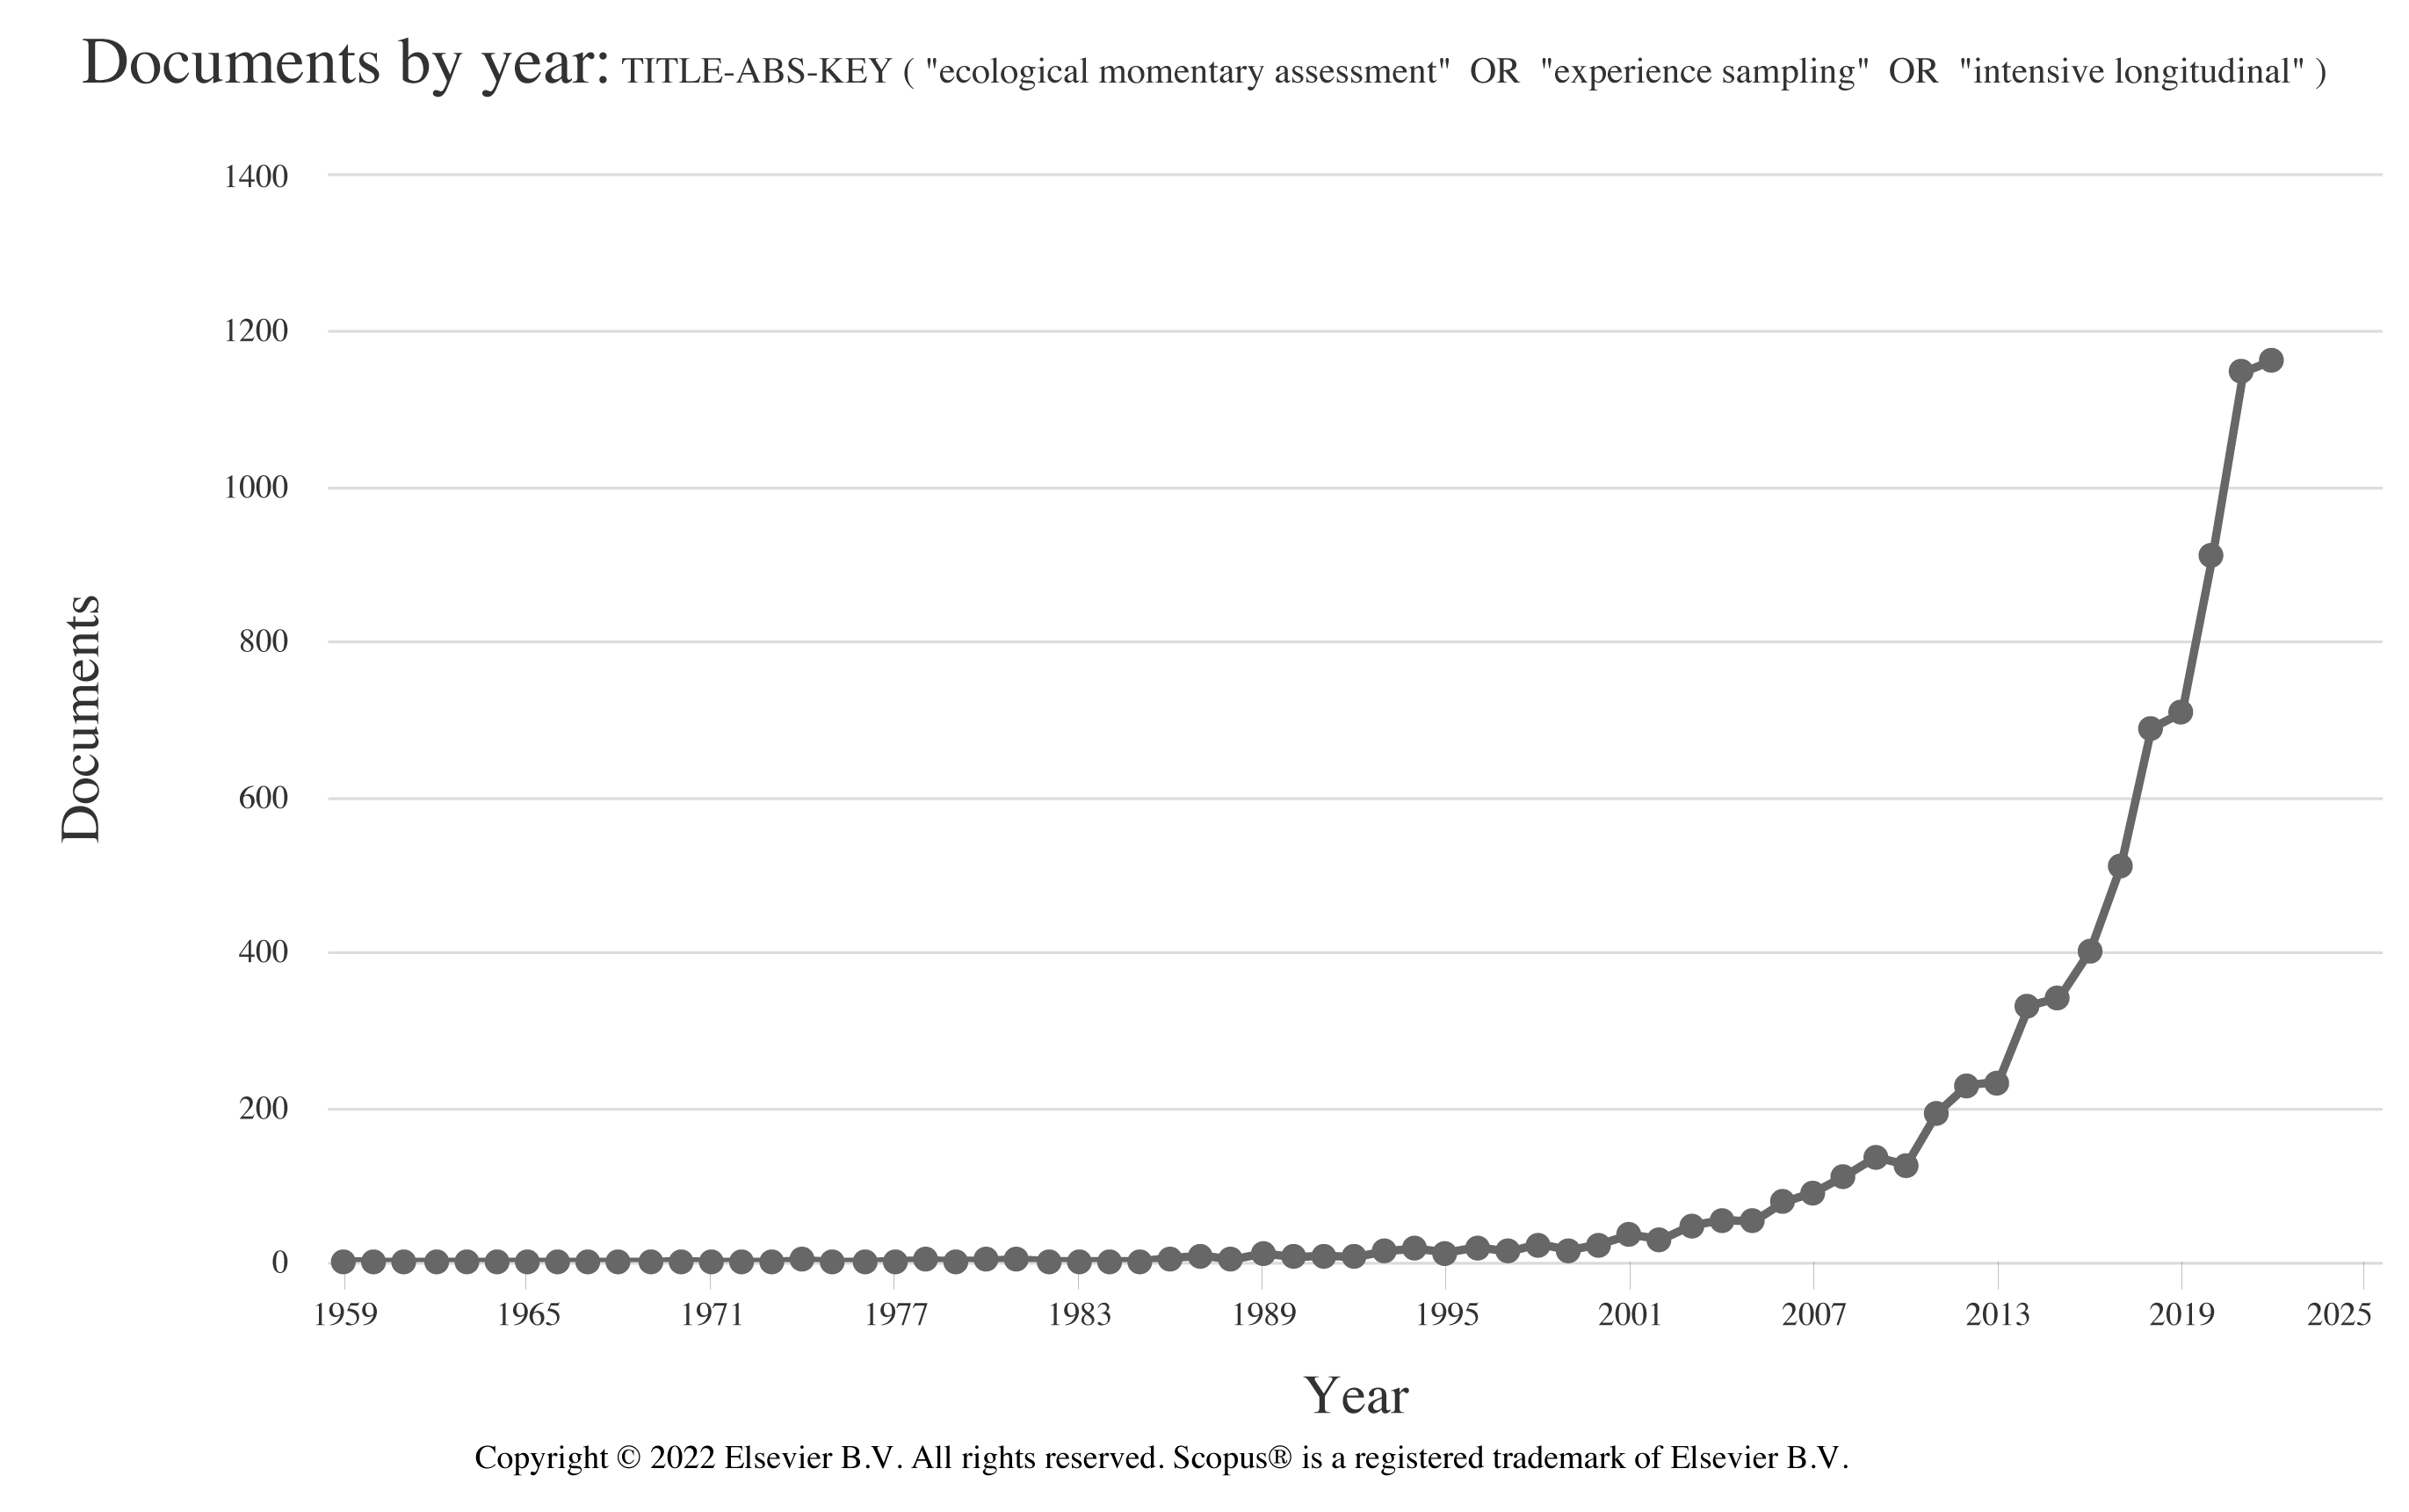
\includegraphics[width=\textwidth]{figures/Scopus-ESM-Development.png}
  \caption*{Note: \\
  Search Terms: `( "ecological momentary assessment"  OR  "experience sampling"  OR  "intensive longitudinal")' in Title, Abstract, or Keyword.}
\end{figure}

Time series clustering has a number of conceptual use cases with psychological data. Prime among them is the ability to reduce the time, variable, and person complexity by extracting and organizing participant-level structures. These reduction and structuring qualities can be essential in detecting phenomena and extracting more abstract functional principles \citep[][]{eronen2021a}. These phenomena and principles can be meaningful differences that distinguish participants in different clusters, as well important patterns, trends, and relationships that participants share within a cluster \citep[e.g.,][]{schrodt2000}. Once distinct groups and patterns have been identified, researchers can examine the extent to which these within-group and between-group structures are associated with other variables of interest, such as personality traits, demographic characteristics, or other psychological constructs \citep[e.g.,][]{monden2022}. Once meaningful and robust structures and patterns are detected, time series clustering can, thus, be used to inform the development of robust theories as well as targeted interventions and therapies for individuals, for example, with mood disorders and other psychological conditions \citep[e.g.,][]{borsboom2021, eronen2020}.


%Time-series clustering has been extremely common in other empirical fields, including analyses of astronomical, meteorological, and aviation pathways, biological and medical developments, as well as energy and finance patterns \citep{Aghabozorgi2015}. But also for psychological data, time-series clustering has recently become more common \citep[e.g.,][]{ernst2021}.

However, while clustering can be incredibly useful, arriving at these clusters critically depends on two core challenges. 

this means time series clustering critically depends on making time series comparable to 
identify key (dis)similarities and then accurately distinguishing different groups \citep[e.g.,][]{Aghabozorgi2015}.

The main aim of time series clustering is to inductively group participants in such a way that the dynamics of some variable(s) have maximum similarity for individuals in the same group, and minimum similarity for individuals in different groups \citep[e.g.,][]{Aghabozorgi2015}. In practice, this means time series clustering critically depends on identifying similarities or dissimilarities in time series and then accurately distinguishing different groups \citep[e.g.,][]{Aghabozorgi2015}. Broadly speaking, time series (dis-)similarity can be approximated by either comparing the raw time series or by comparing some numerical representation of the time series (e.g., \citealp[]{liao2005}; see \fgrref{fig:tsClustTax} for an illustration). The (dis-)similarity measurements can then be clustered either on their own or as part of the representation estimation (e.g., \citealp[]{denteuling2021}; see `embedded' in \fgrref{fig:tsClustTax}).

\begin{figure}[!hbtp] %hbtp
  \caption{Time Series Clustering Taxonomy}
  \label{fig:tsClustTax}
  \centering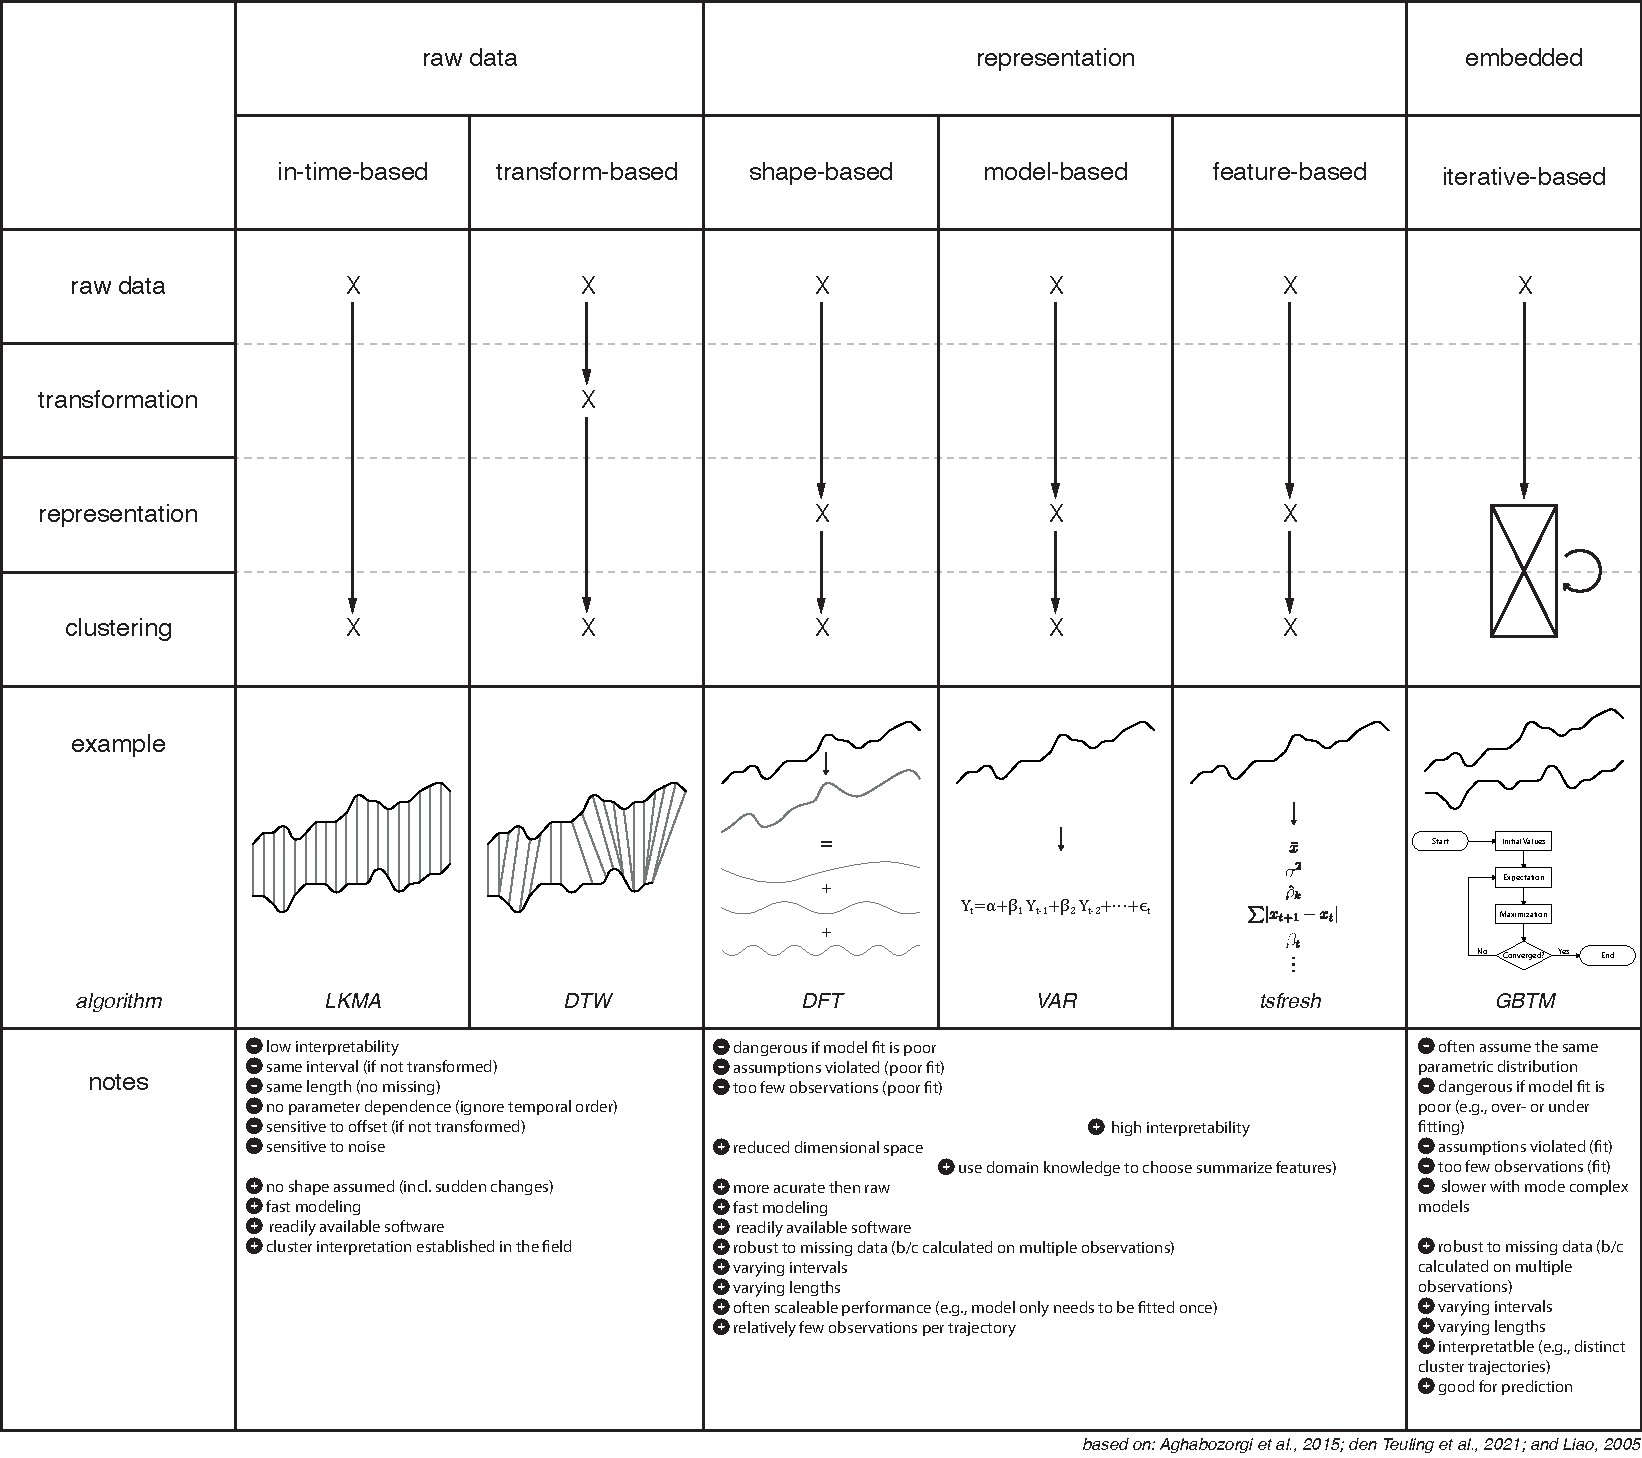
\includegraphics[width=\textwidth]{figures/TS Cluster Flow/tsClustTax.pdf}
  \caption*{Note: \\
  The taxonomy only exemplifies some of the basic differences between a number of common time series clustering approaches. As such, the taxonomy and the notes are neither exhaustive nor complete in distinguishing different approaches. Additionally, terms and labels are used inconsistently across different types of literature and are chosen to avoid overlapping labels.}
\end{figure}

Thus far, one of the most common clustering approaches for ESM data has been to group individuals based on person-specific model parameters --- notably intercepts and slopes from vector autoregression models \citep[VAR; e.g.,][]{ariens2020}. While these model parameters are familiar to researchers in the field, the model-based approach has a number of important shortcomings. Computationally, the number of parameters compounds with increases in variables and lag orders, which tends to result in efficiency and accuracy reduction for most clustering algorithms and is sometimes referred to as the dimensionality curse \citep{altman2018}\footnote{As an illustration of this scalability issue, consider a VAR model of 8 variables that includes the first three lags (i.e., VAR(3)). For each of the 8 variables, we would have 25 parameters --- one intercept and 24 slopes (8 variables * 3 lags each). That compounds to a total of 200 parameters per person (8 variables * 25 parameters).}. But more importantly, using model parameters means that the clustering is restricted by the assumptions and limitations of the statistical model. To take the common VAR model as an example, the model assumes that the time intervals between measurements are identical (i.e., equidistant measurements), it does not allow for missing values, and it assumes that the means as well as variances of the variables do not change over time \citep[i.e., stationarity assumption;][]{lutkepohl2005}. 

These shortcomings, however, stand in sharp contrast with the types of data researchers commonly collect and common research interests in the field. Psychological researchers might, for example, collect data based on the occurrence of natural events, which tends to result in non-equidistant measurements \citep[e.g.,][]{myin-germeys2018, hamaker2017} and context-specific missingness that cannot be imputed, for instance, interaction quality perceptions \citep[e.g.,][]{kivela2022, lavori2008}. At the same time, researchers are often specifically interested in non-stationary developments, looking, for example, at how symptom levels and -variations change over time --- often abruptly and non-linearly \citep[][]{bringmann2018b, helmich2020a}. We offer a more extensive discussion of the current challenges that clustering approaches should address in \appref{app:ChallengesAppendix}. In short, the time series clustering repertoire should be extended to approaches that can more flexibly allow for diverse measurement and missingness patterns and can capture non-stationary data, including non-linear trends, also across different time scales.

Importantly, model-based clustering is not the only clustering approach, and model intercepts and slopes are not the only way in which researchers conceptualize and describe time series. A flexible extension of model-based clustering is feature-based clustering \citep[e.g.,][]{Aghabozorgi2015}\footnote{It should be noted that a third option is shape-based clustering, which uses the raw time series and seeks to match different time series by non-linearly stretching and contracting the time axes. Shape-based clustering might be less relevant to many psychological time series because the forced alignment and scaling can, for example, lead to misspecifications \citep[e.g., ][]{faloutsos1994}. Such scaling issues are less of a concern for highly regular and comparable time series such as EEG \citep[][]{huang1985}.}. Whereas model-based clustering is specifically limited to model parameters as time series characteristics, feature-based clustering extends the time series characteristics to virtually any numerical summary of a time series \citep[e.g.,][]{liao2005}. As an illustration of the flexibility of this approach, a commonly used software package for this approach allows users to extract a total of 794 time series features \citep[][]{christ2018}. Time series features can be chosen by the user based on their research question and can, for example, include the mean and standard deviation of a time series, but also linear and non-linear trends, inertia-related features such as auto-correlations, or the stability of the time series \citep[e.g., mean absolute change; e.g.,][]{barandas2020}. Given the flexibility of the feature-based approach, users are able to apply the analysis across multivariate data, feature extraction mitigates issues of non-equidistant and structurally missing data, and the features can capture and compare across non-linear trends at different time scales.

\section{Feature-based Time Series Clustering}

\subsection{Features of Psychological Time Series}
There are hundreds of possible ts features 

\citet{kuppens2017} originally proposed (1) variability, (2) co-variance or ICC, (3) inertia, and (4) cross-lagged correlations. These features were then extended and formalized by \citet{krone2018} into (1) within-person variance, (2) innovation, (3) inertia or autocorrelation, (4) cross-lagged regression parameters, (5) covariances as granularity, and (6) mean intensity. \citet{krone2018} were even able to use these features to cluster study participants.

\citet{dejonckheere2019} discuss (1) mean, (2) variance, (3) relative variance, (4) instability, (5) inertia / autoregression, (6) interdependence / network density, (7) granularity or differentiation / ICC, (8) correlation, and (9) diversity / Gini coefficient. 

Outside the psychological literature, time series features have also included more summaries in terms of measurement distribution, categorical states, and, importantly, nonlinear developments. 

\citet{kiwuwa-muyingo2011} proposed to extract clinically meaningful states for medical adherence data. 

\citet{wang2006} propose a set of nine statistical features for describing a trajectory: (1) trend, (2) seasonality, (3) periodicity, (4) skewness, (5) kurtosis, (6) serial correlation, (7) non-linearity, (8) self-similarity, and (9) chaos. This selection was also used by \citep{fulcher2013}. \citet{adya2001} proposed a total of 28 features relevant for forecasting, which largely fit within the selection proposed by \citet{wang2006}.


Fortunately, past conceptual and empirical efforts offer valuable discussions of common time series features in psychological research. While the final selection of features should always be driven by the research questions and field-specific conventions, we can build a practical toolbox of meaningful time series features for psychological data. In particular, we propose to focus on six features based on common psychological research questions and recent works on affect dynamics \citep[e.g.,][]{dejonckheere2019, kuppens2017, adya2001}. An overview of the proposed features, their substantive interpretations, and mathematical operationalizations is available in \tblref{tab:esmFeatures}.

The first two features are a person's \textit{central tendency} and \textit{variability}. Familiar statistics from probability theory, the two features sit at the heart of many fundamental psychological questions. ``Are some people happier than others?'' (i.e., difference in central tendency), and "Are people settled in their attitudes towards migrants or do they fluctuate over time?'' (i.e., difference in variability). Mathematically, both features have parametric and robust options to choose from (e.g., parametric: mean and standard deviation; robust: median and median absolute deviation). 

The third and fourth features describe the structure of the variability within the time series. In particular, \textit{(in)stability} captures the average change between two consecutive measurements. Do changes tend to be slow and gradual or fast and abrupt? Mathematically, (in)stability measurements often look at the average change between two consecutive measurements. \textit{Inertia} describes how much a measurement carries over to future measurements. There are two main ways in which experiences tend to be connected to future experiences --- resistance to change and seasonality. Both forms of inertia relate to different types of research questions. ``Do patients stay in a depressed mood for several measurements?'' (i.e., stability-inertia), and ``Do participants drink more alcohol on Fridays?'' (i.e., periodicity-inertia). Both forms of inertia are often measured using autocorrelations with either a lag-1 (stability-inertia) or the lag of the seasonality (e.g., seven days). Periodicity-inertia can additionally be captured using wave patterns (e.g., fourier or wavelet transformation).

The final two features are linear and nonlinear trends. \textit{Linear trends} are a common research interest for longitudinal data. ``Do patient symptoms improve?'' or ``Does worker productivity decline?'', are familiar types of research questions. Mathematically, such linear trends are commonly captured using (piecewise) linear regression coefficients. \textit{Nonlinear trends} are important in two regards. Firstly, nonlinearity is a deviation from linear trends and secondly, the shape and structure of the nonlinear trend. Questions like ``Is the development of anxiety a nonlinear process?'' are mathematically captured using nonlinearity parameters such the bicoherence metrics \citep{cuddy2009}. The structure of nonlinear trends is often mathematically captured using polynomial coefficients or more broadly by how wiggly the line is (e.g., estimated degrees of freedom of GAM spline models; similar to the number of spikes \citealp[]{caro-martin2018}). 

This selection of the proposed six time-series features is in no way exhaustive or imperative. Both using a purely data-driven approach or selecting other aspects to summarize the time series are legitimate options. The list seeks to offer a practical toolbox of features that are common and meaningful to psychological research questions and -practice (see \tblref{tab:esmFeatures} for a more complete overview).


\paragraph{Central Tendency}

\paragraph{Variability}

\paragraph{(In)stability}

\paragraph{Inertia and Periodicity} self-similarity, seasonality, periodicity, inertia

\paragraph{Linear Trend}

\paragraph{Nonlinearity}

\subsection{Analysis Steps}

------------------------

NOTES:

model based clustering: \citep{bulteel2016, stefanovic2022}

parameter-based clustering: VAR \citep{ernst2021} splines \citep{axen2011} 

sort of feature-based clustering in psych \citep{heylen2016} as well as \citep{krone2018}

clustering in reduced space \citep{timmerman2013}

------------------------

The feature-based clustering can be structured into four main steps \citep{rasanen2009, wang2006}. (1) The selection and preparation of the input variables, (2) the extraction of the features that describe the time series, (3) an optional feature reduction step if there are too many data points for the clustering algorithms, and (4) the actual clustering of the time series features. We provide a conceptual overview that can be used alongside this section in \fgrref{fig:TSCFlow}. 

\begin{figure}[!ht] % \begin{figure*}[hbtp] <-- on its own page
  \caption{Flowchart Feature-Based Time Series Clustering in Psychology}
  \label{fig:TSCFlow}
  \centering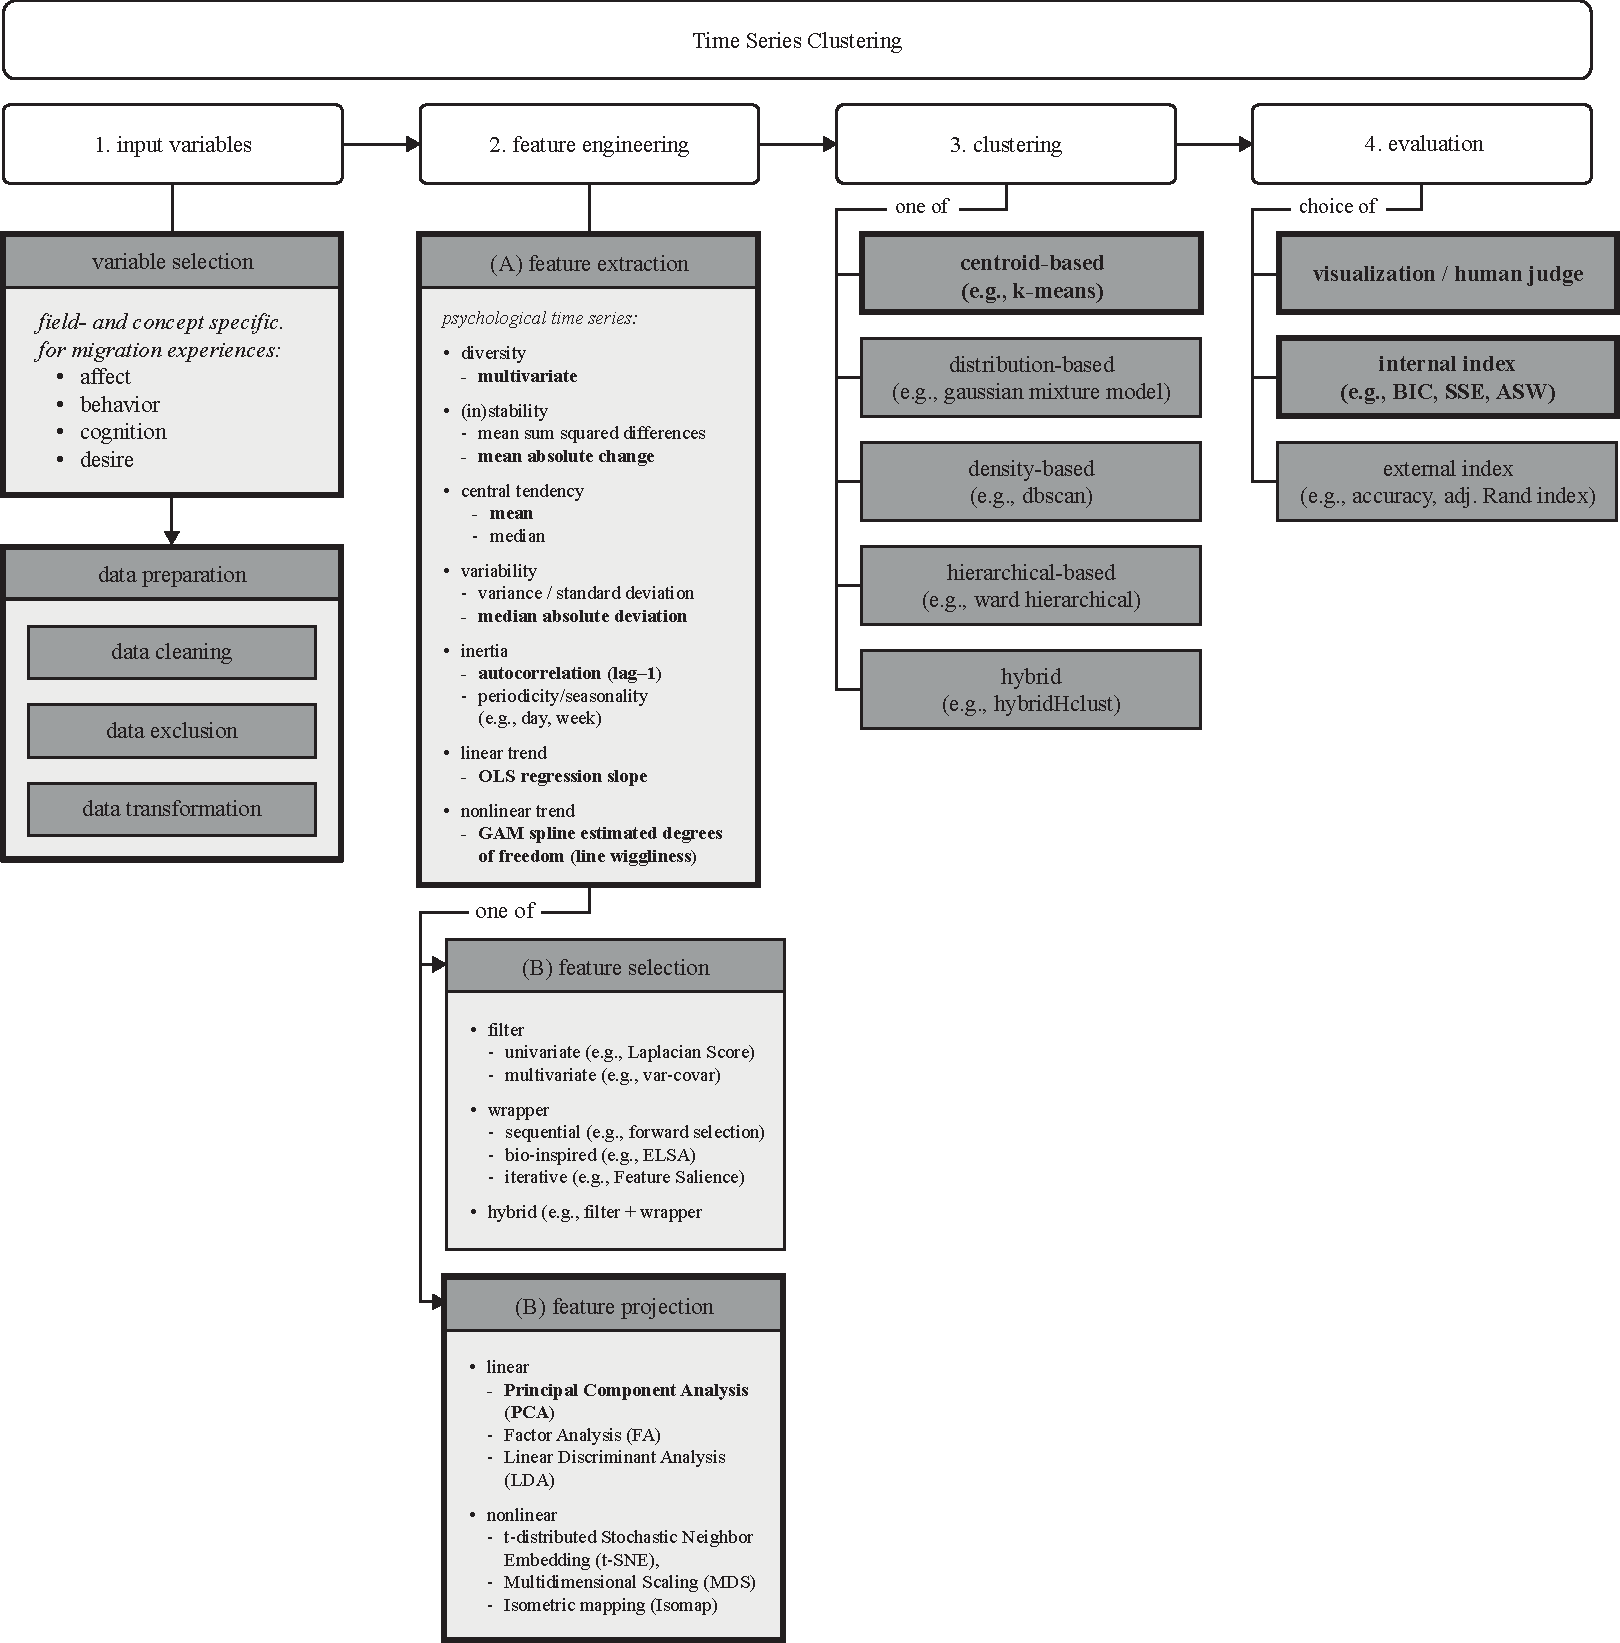
\includegraphics[width=\textwidth]{figures/TS Cluster Flow/TimeSeriesClusterFlowSelection.pdf}
  \caption*{Note: \\
  Choices selected for illustration in this manuscript are marked in bold.}
\end{figure}

\paragraph{Input variables}
Time series clustering starts with the selection and preparation of the variables of interest. While the selection will necessarily be field- and concept-specific, there are a few conceptual and methodological issues that should be considered. Conceptually, the included variables should adequately capture the concept of interest and should be meaningful to the understanding of the time series. There are, for example, calls that emotion dynamics should be assessed with a repertoire of positive and negative emotions \citep[e.g.,][]{dejonckheere2019}, migration experiences are fully captured with affect, behavior, cognition, and desire measurements \citep[e.g.,][]{Kreienkamp2022d}, and many health developments are commonly captured within the biopsychosocial domains \citep[e.g.,][]{suls2004}. At the same time, however, the added number of variables can become a methodological concern. Not only can redundant and irrelevant variables diminish the quality of the analyses, but with intensive longitudinal data the number of data points compounds across participants, measurement occasions, and variables so that additional variables can make many of the following steps substantially more difficult (also see \fgrref{fig:TSCFlowN}). 

\begin{figure}[!ht] %hbtp
  \caption{Exemplary Flowchart of Data Points in Feature-Based Time Series Clustering}
  \label{fig:TSCFlowN}
  \centering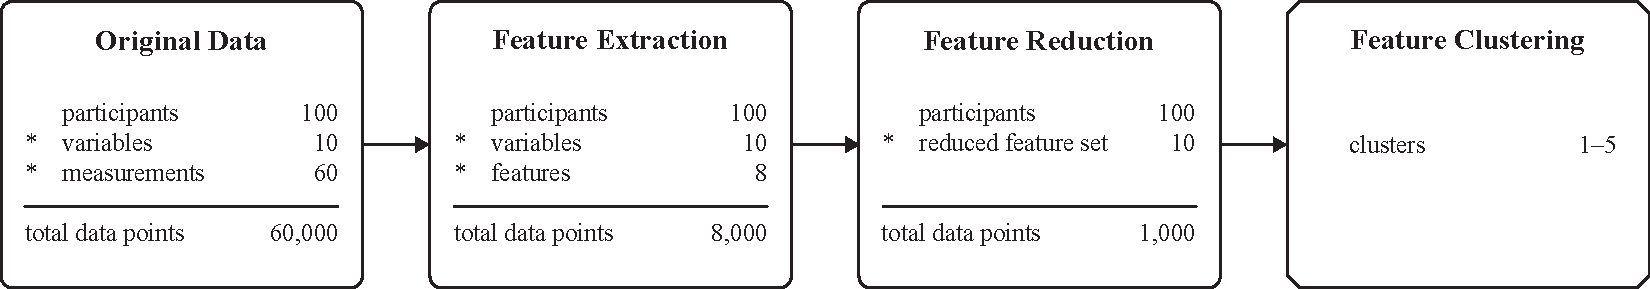
\includegraphics[width=\textwidth]{figures/TS Cluster Flow/tsClustFlowN.pdf}
  \caption*{Note: \\
  The presented number of participants, variables, and measurement occasions are somewhat arbitrary but generally represent common sample sizes found within the literature. Also the number of extracted clusters is presented for illustrative purposes only.}
\end{figure}

Once the important variables have been selected, the data needs to be prepared for the analysis steps. Importantly, this not only means validating and cleaning the data (e.g., re-coding, removing duplicate or unwanted measurements) but also making the time series comparable. Two important steps are making the time-frames and response scales comparable across participants. Extracting features that describe the development of a month for one participant but 90 days for another participant might not be comparable for some psychological phenomena. This comparability is important on a conceptual level but the difference in data availability might also influence the clustering steps, where the participant with the shorter measurement period would, for example, have a larger number of missing values. It is thus generally advised to reduce the data to a common and comparable time frame. 

\paragraph{Feature extraction}
The main aim of feature extraction is to describe the most important and meaningful aspects of a time series. There are, however, hundreds of possible features to describe psychological time series \citep[e.g., tsfresh][]{christ2018}. One approach to choosing relevant features would be to extract a large number of features and then assess which features are most effective at capturing differences in the time series. However, such an approach is not always advisable for psychological time series. For one, features should reduce the data dimensionality --- it would thus not necessarily be advisable to describe 60 ESM measurements with 180 time series features. More importantly, however, careful feature extraction can be crucial in the interpretability and explainability of the results. This is particularly the case when features have a conceptual or psychological meaning. Taking the concept of well-being as an example, psychologists might be interested in whether certain participants tend to have higher well-being in general (i.e., mean) or whether some participants fluctuate between extremely high and low well-being (i.e., variance). But psychologists might not necessarily be interested in the exact time point after which 50\% of the summed well-being values lie (i.e., relative mass quantile index) or how much different sine wave patterns within the well-being data correlate with one another (i.e., cross power spectral density). We would, thus, strongly advocate for a careful selection of time series features that are meaningful to the field and concepts.

%\begin{table}%[hbt]
\begin{sidewaystable*}[!hbtp]
    \centering
    \caption{Examples of Features for Psychological Time Series.}
    \label{tab:esmFeatures} 
    \begin{tabular}{
    >{\raggedright\arraybackslash}p{0.15\linewidth} 
    >{\raggedright\arraybackslash}p{0.35\linewidth} 
    >{\raggedright\arraybackslash}p{0.25\linewidth} 
    >{\raggedright\arraybackslash}p{0.20\linewidth}
    }
        \hline 
        Time Series Feature & Substantive Interpretation & Example Operationalizations & Formulas, refs, ...? \\ 
        \hline \\ [-0.5em]
        
        %Diversity \newline \hl{(drop this \& keep in var. selection only?)} & 
        %Multivariate measurement of concepts (e.g., affect-behavior-cognition-desire, or bio-psycho-social) \linebreak & 
        %-----\linebreak  & 
        %{\centering --- ? ---\par} \\
        
        Central Tendency \linebreak & 
        Average level of the experience across the entire measurement period. \linebreak & 
        \vspace{-1em}
        \begin{itemize}[nosep,leftmargin=*,label={--}]
            \item mean
            \item median
            \item mode
        \end{itemize} \linebreak  & 
        {\centering --- ? ---\par} \\ 
        
        Variability & 
        Describes the average deviation from the central tendency across the entire measurement period. \linebreak & 
        \vspace{-1em}
        \begin{itemize}[nosep,leftmargin=*,label={--}]
            \item standard deviation
            \item variation coefficient
            \item median absolute deviation
        \end{itemize} \linebreak & 
        {\centering --- ? ---\par} \\ 
        
        (In)stability & 
        Describes the average change between two consecutive measurements of the experience. \linebreak & 
        \vspace{-1em}
        \begin{itemize}[nosep,leftmargin=*,label={--}]
            \item mean sum squared differences
            \item mean absolute change
            \item Ix instability index
        \end{itemize} \linebreak & 
        {\centering --- ? ---\par} \\ 
        
        Inertia & 
        Describes how much experiences carry over to the future measurements. This includes resistance to change (i.e., carries over to the next measurement) and periodic or seasonal returns (e.g., self-predictive on a daily or weekly basis). \linebreak &
        \vspace{-1em}
        \begin{itemize}[nosep,leftmargin=*,label={--}]
            \item autocorrelation (e.g., lag–1)
            \item fourier coefficients
            \item continuous wavelet transform
        \end{itemize} \linebreak & 
        {\centering --- ? ---\par} \\ 

        Linear Trend & 
        Describes upwards or downwards linear trend of the experience reports. \linebreak & 
        \vspace{-1em}
        \begin{itemize}[nosep,leftmargin=*,label={--}]
            \item OLS regression slope
            \item avg. piecewise linear reg. slope
        \end{itemize} \linebreak & 
        {\centering --- ? ---\par} \\ 
        
        Nonlinearity & 
        Describes the nonlinear structure of the time series. This includes measures that indicate the deviation from the a linear trend as well as nonlinear model parameters. \linebreak & 
        \vspace{-1em}
        \begin{itemize}[nosep,leftmargin=*,label={--}]
            \item GAM spline edf
            \item bicoherence metrics
            \item Langevin polinomial coefficient
        \end{itemize} \linebreak & 
        {\centering --- ? ---\par} \\ 
        
        \hline \\ [-0.75em]
        \multicolumn{4}{p{\linewidth}}{\footnotesize \textit{Note.} The presented features and operationalizations are neither exhaustive nor necessary for feature-based clustering.}
    \end{tabular}
\end{sidewaystable*}


\paragraph{Feature reduction}
Once a meaningful selection of time series features has been extracted for each variable and participant, the total number of data points usually remains too large for most clustering algorithms. As an example, a relatively common scenario would include 10 variables of interest, where 8 time series features are extracted, resulting in 80 features per participant (with a common sample size of 100 participants that would result in a total of 8,000 data points in this hypothetical example). We offer an illustration of the compounding numbers of data points in \fgrref{fig:TSCFlowN}. The difficulty of working with such a large number of dimensions is sometimes termed the `dimensionality curse' \citep[e.g.,][]{altman2018}. To deal with this dimensionality issue, two main approaches have been proposed --- feature selection and feature projection (a full overview of the approaches, methods, and common algorithms is available in \tblref{tab:featureReduction}). 

Feature selections seek to create a subset of the most important features. The many available approaches differ in how they seek to determine the importance of the individual features. Generally speaking, selection methods can be categorized as `filter', `wrapper', or `hybrid' methods. The filter methods, broadly speaking determine important features by identifying irrelevant features (e.g., because features do not capture much information), and identifying redundant features (e.g., because features capture the same information). Wrapper methods on the other hand avoid the feature-based evaluation and focus on the performance of the later model to identify the most important features. A wrapper, thus, compares the performance of models with different feature combinations. Traditional examples of wrappers are forward selection or backward elimination procedures. Because filter methods might not always perform well and wrapper methods are computationally intensive\footnote{Computationally \textit{k} features could be considered in \(2^k – 1\) possible combinations --- for the example of 80 features that would allow for \(1.20 \times 10^{24}\) (over one septillion) combinations.}, hybrid methods seek to combine the two methods and find a balance between computational effort (i.e., efficiency) and performance (i.e., effectiveness). Methods might, for example, use a filter step to reduce the size of features considered in a later wrapper step.

The second general approach to the dimensionality curse has been feature projection. Projection methods are relatively common in psychological research --- including, factor- and principal component analyses. Generally speaking, projection methods seek to transform the many features in such a way that a much smaller number of new variables can accurately capture the variance and structure of the original features (i.e., the data is projected to a lower dimensional space). Commonly, this is achieved using linear transformations (e.g., principal component analysis), or more complex nonlinear transformations (e.g., t-SNE). Generally speaking, feature selection procedures have the benefit that they retain the interpretable feature labels directly and immediately indicate which features were most informative in the sample. Feature projection methods, on the other hand, tend to be more generalized and are more readily available.

%\begin{table}%[hbt]
\begin{sidewaystable*}[!hbtp]
    \centering
    \caption{Examples of Feature Reduction Approaches and Methods.}
    \label{tab:featureReduction} 
    \begin{tabular}{
    >{\raggedright\arraybackslash}p{0.08\linewidth} 
    >{\raggedright\arraybackslash}p{0.08\linewidth} 
    >{\raggedright\arraybackslash}p{0.54\linewidth} 
    >{\raggedright\arraybackslash}p{0.25\linewidth}
    }
        \hline 
        Approach & Method & Intuitive Description & Algorithm Examples \\ 
        \hline \\ [-0.5em]
        
        Selection \linebreak & 
        filter \linebreak & 
        Features are selected individually or jointly based on selection criteria. One common selection criterion is the amount of information and (unique) variance a feature captures. Univariate methodologies are able to identify irrelevant features (i.e., because features do not capture much information), multivariate methods additionally allow to remove redundant features \citep[i.e., because features capture the same information][]{yu2004}. \linebreak &
        \vspace{-1em}
        \begin{itemize}[nosep,leftmargin=*,label={--}]
            \item univariate filter (e.g., Laplacian Score)
            \item multivariate filter (e.g., variance-covariance)
        \end{itemize}
         \linebreak \\ 
        
        \linebreak & 
        Wrapper \linebreak & 
        Wrapper methodologies run models with different feature combinations and compare performance. Because the selection process is essentially a search problem this method is computationally intensive. Traditionally wrappers have used forward selections or backward eliminations but recently alternative approaches have been proposed based such as ant colony and swarm intelligence paradigms \citep[e.g., see][]{tang2014}. \linebreak &
        \vspace{-1em}
        \begin{itemize}[nosep,leftmargin=*,label={--}]
            \item sequential (e.g., forward selection)
            \item bio-inspired (e.g., ELSA)
            \item iterative (e.g., feature salience)
        \end{itemize}
         \linebreak \\ 
        
        \linebreak & 
        hybrid \linebreak & 
        Hybrid selection methodologies combine filter and wrapper methodologies to avoid the shortcomings of the individual methods. An initial filter step selects candidate features (efficiency) and a subsequent wrapper ensures high performance \citep[effectiveness; e.g.,][]{alelyani2014}. \linebreak &
        \vspace{-1em}
        \begin{itemize}[nosep,leftmargin=*,label={--}]
            \item filter + wrapper (e.g., Calinski-Harabasz Index)
        \end{itemize}
        \linebreak \\

        Projection \linebreak & 
        linear \linebreak & 
        Linear dimensionality reduction methodologies use linear transformations of the original data to stretch and shift the data in such a way that the data can be `projected' to a lower dimensional space without loosing too much information. These methods are well-established, tend to be fast, and usually do not need much conceptual input from the user \citep[][]{cunningham2015}. \linebreak &
        \vspace{-1em}
        \begin{itemize}[nosep,leftmargin=*,label={--}]
            \item Principal Component Analysis (PCA)
            \item Factor Analysis (FA)
            \item Linear Discriminant Analysis (LDA)
        \end{itemize}
         \linebreak \\
        
        \linebreak & 
        nonlinear \linebreak & 
        Nonlinear dimensionality reduction methods also seek to map high-dimensional data to a lower dimensional space. However, nonlinear methods have been developed to preserve the local and global structure of more complex multidimensional patterns \citep[e.g.,][]{lee2007}.
        \linebreak &
        \vspace{-1em}
        \begin{itemize}[nosep,leftmargin=*,label={--}]
            \item t-distributed Stochastic Neighbor Embedding (t-SNE)
            \item Multidimensional Scaling (MDS)
            \item Isometric mapping (Isomap)
        \end{itemize}
        \linebreak \\
        
        \hline \\ [-0.75em]
        \multicolumn{4}{p{\linewidth}}{\footnotesize \textit{Note.} The presented dimensionality reduction methods and -approaches are neither exhaustive nor necessary for feature-based clustering. Notable additional approaches are `embedded selection methods' that filter as part of the model estimation procedure (e.g., mixture models) and `network-based projection methods' that use neural networks to reduce dimensions (e.g., autoencoders).}
    \end{tabular}
\end{sidewaystable*}


\paragraph{Feature clustering}
For feature-based time-series clustering, the main aim is to organize participants into groups so that the features of participants within a group are as similar as possible, while the features of people in different groups are as different as possible. The crux of clustering is, thus, to have clearly defined and effective measurements of (dis)similarity. Most of the clustering algorithms used today use some form of distance measurement to optimize group assignment (or similarity measurement for qualitative features). While others have produced excellent overviews of the many clustering approaches available \citep[e.g.,][]{xu2015}, we will briefly introduce some of the more readily available approaches suitable for most time series feature data. The well-established and readily available clustering approaches can, broadly speaking, be categorized as based on (1) centroids, (2) distributions, (3) density, (4) hierarchies, or (5) a combination thereof (see \tblref{tab:clusterApproaches}). 

Each of these approaches can be a valuable clustering approach for time series feature data and users will usually have to make an informed decision based on the structure of their data as well as an appropriate weighing of accuracy and efficiency. As an example, under ideal conditions, all approaches are likely to suggest very similar clusters. However, when the shapes of clusters, for example, become more complex in a multi-dimensional space, density-based or hierarchy-based approaches that allow for more bottom-up clustering are likely to be more accurate. Yet, with higher numbers of participants and features, both density- and hierarchy-based approaches may perform less well and the more efficient centroid-based methods might be more effective. Similarly, several of the proposed time series features are statics that are generated from Gaussian distributions and a distribution-based algorithm might be ideally suited to separate such distributions \hl{(Corduas \& Piccollo, 2008)}. Yet, in cases where mis-specifications are costly, a method with fewer assumptions might be more advisable. 

There is thus, unfortunately, no one-size-fits-all solution to clustering. On the bright side, however, the thriving methodological developments in the clustering literature offer a wide variety of options that offer prospects even for extremely large and complex data sets. We provide a short intuitive explanation for common approaches, together with some of their characteristics and example algorithms in \tblref{tab:clusterApproaches}. For our own illustration, we have chosen that centroid-based k-means clustering. While k-means comes at the expense of high accuracy with more complex cluster shapes, we specifically chose k-means because it is an extremely efficient method that works well with large participant- and feature numbers without making too many restrictive assumptions about the shape of the data. K-means is also well-established within the research community and has been readily implemented in many statistical software packages. Additionally, many of the feature selection methods have specifically been designed for the well-established k-means algorithm. As such, the k-means offers a good starting point for many psychological researchers and the method should be generalizable across a relatively wide variety of projects.

\paragraph{Cluster Performance Evaluation}

PARAGRAPH ON PERFORMANCE METRICS (incl., cross-validation?)

incl., finding cluster prototypes:
1. The medoid sequence of the set. 2. The average sequence of the set. 3. The local search prototype

External evaluation measures: These measures require knowledge of the true class labels and are used to compare the cluster assignments to the true class labels. Examples include accuracy, F-measure, adjusted Rand index, mutual information, and normalized mutual information.

Internal evaluation measures: These measures do not require knowledge of the true class labels and are used to evaluate the quality of the clusters based on the characteristics of the data itself. Examples include silhouette coefficient, Calinski-Harabasz index, Davies-Bouldin index, and the Elbow method.

PARAGRAPH ON REPORTING \citep[e.g.,][]{vandeschoot2017}

%\begin{table}%[hbt]
\begin{sidewaystable*}[!hbtp]
    \centering
    \caption{Common Clustering Approaches.}
    \label{tab:clusterApproaches} 
    \begin{tabular}{
    >{\raggedright\arraybackslash}p{0.15\linewidth} 
    >{\raggedright\arraybackslash}p{0.40\linewidth} 
    >{\raggedright\arraybackslash}p{0.28\linewidth} 
    >{\raggedright\arraybackslash}p{0.12\linewidth}
    }
        \hline 
        Approach & Description & Characteristics & Examples \\ 
        \hline \\ [-0.5em]
        
        centroid-based \linebreak & 
        Chooses a pre-defined number of potential cluster centers in the feature space and assigns participants to closest center. Then, iteratively, moves the centers until a convergence criterion is met (e.g., all distances to centers minimized).
        \linebreak &
        \vspace{-1em}
        \begin{itemize}[nosep,leftmargin=*,label={--}]
            \item[\scriptsize\faPlusCircle] simple and efficient
            \item[\scriptsize\faPlusCircle] no assumptions
            \item[\scriptsize\faPlusCircle] well implemented
            \item[\scriptsize\faMinusCircle] may struggle with complex shapes
            \item[\scriptsize\faMinusCircle] sensitive to initial values and outliers
            %\item[\scriptsize\faMinusCircle] not suitable for non-convex data, relatively sensitive to the outliers, easily drawn into local optimal, the number of clusters needed to be preset, and the clustering result sensitive to the number of clusters \citep{xu2015}.
        \end{itemize}\linebreak & 
        \vspace{-1em}
        \begin{itemize}[nosep,leftmargin=*,label={--}]
            \item k-means
            %\item fuzzy c-means
            %\item CLARA
            \item PAM
        \end{itemize}\linebreak \\ 
        
        distribution-based \linebreak & 
        Assumes that the data points belong to one of several specific distributions (e.g., Gaussian distributions). Data points that fit to a distribution-based expectation are given higher probability of belonging to that distribution. We can then iteratively check with which model parameters the data points best fit within given number of distributions.
        \linebreak &
        \vspace{-1em}
        \begin{itemize}[nosep,leftmargin=*,label={--}]
            \item[\scriptsize\faPlusCircle] probabilistic
            \item[\scriptsize\faPlusCircle] well supported
            \item[\scriptsize\faMinusCircle] time intensive
            \item[\scriptsize\faMinusCircle] distribution and parameter sensitive
        \end{itemize}\linebreak & 
        \vspace{-1em}
        \begin{itemize}[nosep,leftmargin=*,label={--}]
            \item GMM
            %\item negative binomial model-based
            \item DBCLASD
        \end{itemize}\linebreak\\ 
        
        density-based \linebreak & 
        Assumes that clusters are regions where several data points are relatively close together (i.e., high density). Based on what is considered a dense region (e.g., radius of a region and minimum number of points the radius), points can be either be assigned to one of the clusters or be considered too far away from a dense region. \linebreak &
        \vspace{-1em}
        \begin{itemize}[nosep,leftmargin=*,label={--}]
            \item[\scriptsize\faPlusCircle] efficient
            \item[\scriptsize\faPlusCircle] no shape assumption
            \item[\scriptsize\faPlusCircle] do not assign outliers 
            \item[\scriptsize\faMinusCircle] may struggle with uneven densities
            \item[\scriptsize\faMinusCircle] sensitive to high dimensionality
        \end{itemize}\linebreak & 
        \vspace{-1em}
        \begin{itemize}[nosep,leftmargin=*,label={--}]
            \item DBSCAN
            \item OPTICS
        \end{itemize}\linebreak\\ 

        %graph-based \linebreak & 
        %``realized on the graph where the node is regarded as the data point and the edge is regarded as the relationship among data points'' \citep{xu2015} \linebreak &
        %\vspace{-1em}
        %\begin{itemize}[nosep,leftmargin=*,label={--}]
        %    \item[\scriptsize\faPlusCircle] efficient and accurate
        %    \item[\scriptsize\faPlusCircle] no shape assumption
        %    \item[\scriptsize\faMinusCircle] sensitive to graph complexity
        %\end{itemize}\linebreak & 
        %\vspace{-1em}
        %\begin{itemize}[nosep,leftmargin=*,label={--}]
        %    \item MST-based
        %    \item CLICK
        %\end{itemize}\linebreak\\ 

        hierarchy-based \linebreak & 
        Builds a hierarchy of cluster by step-wise combining the closest two clusters (bottom-up; agglomerative) or top down dividing the data into smaller clusters that maximize distances (top-down; divisive).
        \linebreak &
        \vspace{-1em}
        \begin{itemize}[nosep,leftmargin=*,label={--}]
            \item[\scriptsize\faPlusCircle] flexible number of clusters
            \item[\scriptsize\faPlusCircle] no shape assumption 
            \item[\scriptsize\faMinusCircle] best with small number of cases
            \item[\scriptsize\faMinusCircle] no reversal of assignments
        \end{itemize}\linebreak & 
        \vspace{-1em}
        \begin{itemize}[nosep,leftmargin=*,label={--}]
            \item Chameleon
            \item CURE
        \end{itemize}\linebreak \\ 
        
        hybrid \linebreak & 
        Usually combines different approaches, which combine the strength of the complementary approaches. Oftentimes the combination also increases efficiency. \linebreak &
        \vspace{-1em}
        \begin{itemize}[nosep,leftmargin=*,label={--}]
            \item[\scriptsize\faPlusCircle] avoids individual shortcomings
            \item[\scriptsize\faMinusCircle] less readily available
        \end{itemize}\linebreak & 
        \vspace{-1em}
        \begin{itemize}[nosep,leftmargin=*,label={--}]
            \item DD-means
            \item hybridHclust
        \end{itemize}\linebreak\\ 
        
        \hline \\ [-0.75em]
        \multicolumn{4}{p{\linewidth}}{\footnotesize \textit{Note.} The presented clustering approaches and algorithms are neither exhaustive nor necessary for feature-based clustering. Notably, recently innovations have been made based on graph-, fractal-, swarm, and quantum theory \citep[for a more in-depth review see][]{xu2015}.}
    \end{tabular}
\end{sidewaystable*}


\section{Empirical Illustration}
To illustrate common use cases of feature-based time series clustering with psychological ESM data, we apply the clustering process to a recent set of studies that collected diverse concepts with context-specific measurements. The illustration specifically uses data from research on migration experiences, where researchers have started using ESM data to follow the daily interactions of migrants with the cultural majority groups \citep[e.g.,][]{Keil2020}. This new type of research comes as a response to prominent reviews, which have called for more longitudinal \citep[e.g.,][]{Ward2019} and real-world data \citep[e.g.,][]{McKeown2017}. At the same time, conceptual works have pushed for more diverse assessments of migration experiences, including motivational, affective, cognitive, and behavioral aspects \citep[e.g.,][]{Kreienkamp2022d}. The migration ESM research, thus, offers a good example of the modern ESM data that introduces diverse conceptualizations and more event-specific missingness patterns.

% Methods and Results from RMarkdown render
\subsection{Data}

We used a data set following migration experiences collected by
\citet[][]{Kreienkamp2022b}. The data set consists of three studies that
followed migrants who had recently arrived in the Netherlands in their
daily interactions with the Dutch majority group members. After a
general migration-focused pre-questionnaire, participants were invited
twice per day to report on their (potential) interactions with majority
group members for at least 30 days. The short ESM surveys were sent out
at around lunch (12pm) and dinner time (7pm). After the 30 day study
period participants filled in a post-questionnaire that mirrored the
pre-questionnaire. Participants received either monetary compensation or
partial course credits based on the number of surveys they completed.
For our empirical example we focus on the variables that were collected
during the ESM surveys and were available in all three studies. Full
methodological details are available in the empirical article by
\citet[][]{Kreienkamp2022b}.

\subsubsection{Sample}

The original studies included 207 participants (\(N_{S1}=\) 23,
\(N_{S2}=\) 113, \(N_{S3}=\) 71) with a total of 10,297 measurements.
The studies differed substantially in the maximum length of
participation (\(\text{max}(t_{S1})=\) 63, \(\text{max}(t_{S2})=\) 69,
\(\text{max}(t_{S3})=\) 155). This was likely due to the option to
continue participation without compensation in the later two studies. To
make the three studies comparable in participation and time frames, we
iteratively removed all measurement occasions and participants that had
more than 45\% missingness
\citep[which was in line with the general rcecommendation for data that might still need to rely on imputations for later model testing][]{Madley-Dowd2019}.
This procedure let to a final sample of 157 participants, who jointly
produced 8,132 measurements. Importantly, both the participant
repsonse-patterns and the time frame were now a lot more comparable
(\(\text{max}(t_{S1})=\) 61, \(\text{max}(t_{S2})=\) 60,
\(\text{max}(t_{S3})=\) 67). For a full overview of the data reduction
procedure and study-specific exclusions see Online Supplemental Material
A.

\subsubsection{Variables}

We included 12 variables that were available across all three studies
and captured information about the participant's interactions, as well
as cognitive-, emotional-, and motivational self in relationship with
the majority group. We chose these two aspects in particular because (1)
the interaction-specific information exemplified the structural
missingness issue of modern ESM data and (2) the motivational,
emotional, and cognitive experience offered a diverse conceptualization
of migration experience (beyond behavioral measurements) that is
becoming more common in the literature \citep[][]{Kreienkamp2022d}. Full
methodological details are available in Online Supplemental Material A,
but basic item information, descriptives, and correlations are available
in \tblref{tab:descrWide}.

\subsection{Analysis and Results}

To perform the main analysis on our selected variables, we showcase the
extract--reduce--cluster steps in sequential order. For each of the
steps fully reproducible and annotated code is available in Online
Supplemental A as well as in the accompanying OSF- and GitHub
repositories (REFERENCES).

\subsubsection{Feature extraction}

For the features, we selected and extracted one of each of the features
proposed in \tblref{tab:esmFeatures}. We particularly chose the more
robust median and median absolute deviation (MAD) for central tendency
and variability. Within the variability structure, we chose the slightly
more intuitive mean absolute change (MAC) for stability and stayed with
the common lag--1 autocorrelation for inertia. For the trend summaries,
we chose the overall linear regression slope to describe the linear
trend and we summarized the nonlinear trend with the estimated degrees
of freedom of an empty GAM spline model (edf) --- the edf summarizes the
\textit{wiggliness} of the spline trend line. We chose these features in
particular because we consider them to be the most broadly applicable
features. We also extracted the participant's number of completed ESM
measurements to ensure that the clusters are comparable in that regard.
We provide an R-function that automatically extracts and prepares a
large selection of the time series feature operationalizations presented
in \tblref{tab:esmFeatures} in our GitHub repository (see the
\texttt{featureExtractor} function).

After the feature extraction, we found that about 1.40\% of the
extracted features are missing across the 72 features per participant.
This might, for example, happen if participants do not have two
subsequent measurements with outgroup interactions, so that an
autocorrelation with lag-1 cannot be calculated for the contact-specific
variables. The small number of missing values indicates that the
feature-based approach indeed largely avoids the structural missingness
issue. The few missing values can, however, be an issue for some feature
reduction or feature clustering algorithms. We, thus, impute the missing
feature values with a single predictive mean matching imputation using
the MICE library.

\subsubsection{Feature reduction}

For the feature reduction, we chose the common
\textit{principal component analysis} (PCA). Some of the more
tailor-made feature selection algorithms can be more accurate in
reducing the feature dimensionality and might retain feature importance
information more directly, depending on the specific data structure.
However, PCAs have the distinct benefit that they are well-established
within the psychometric literature and can broadly be applied to a wide
variety of studies in an automatize manner. As our aim is to present a
general illustration that can also be adopted for more general data
descriptive uses, we present the workflow using a PCA here but we
encourage users to consider more specialized methods as well.

To use the principal component analysis with our extracted time series
features, we first standardize all features across participants to
ensure that all features are weighted equally. We then enter all 72
features into the analysis. The PCA will use linear transformations in
such a way that the first component captures the most possible variance
of the original data (e.g., by finding a vector that maximizes the sum
of squared distances). The following components will then use the same
method to iteratively explain the most of the remaining variance while
also ensuring that the components are linearly uncorrelated. In
practice, this meant that the PCA decomposed the 72 features into 72
principal components but now (because of the uncorrelated linear
transformations) the first few principal components will capture a
majority of the variance. We can then decide how much information (i.e.,
variance) we are willing to sacrifice for a reduced dimensionality. A
common rule of thumb is to use the principal components that jointly
explain 70--90\% of the original variance (i.e., cumulative percentage
explained variance). For our illustration we select the first 27
principal components that explain 80\% of the variance in the original
72 features (reducing the dimensionality by 62.50\%). For the extracted
principal components we save the 27 PC-scores for each participant
(i.e., the participants' coordinates in the reduced dimensional space).

We would like to comment on two practical matters when using principal
components --- the amount of dimensionality reduction and the
interpretation of the principal components. As for the expected
dimensionality reduction, given its methodology, PCAs tend to `work
better' at reducing dimensions with (highly) correlated variables. Thus,
with a set of very homogeneous variables and features users will need
less principal components to explain a large amount of variance, while a
more diverse set of variables and features will tend to require more
principal components to capture the same amount of variance. Our 27
principal components are still a relatively high number of variables but
this is not surprising as we chose a diverse conceptualization and a
diverse set of time series features. As for the interpretability, PCA
allows users to extract information on the meaning of the principal
components. In particular, because the principal components are linear
combination of original features, users can extract the relative
importance of each feature for the extracted principal components (i.e.,
the eigenvectors). While this can be useful in understanding the
variance in the original data or help with manual feature selection, we
use the PCA purely to reduce the dimensionality for the clustering step.
Instead of relying on the principal components, we use the original
features of interest to interpret the later extracted clusters. We
particularly advocate for such an approach if the original features were
chosen for their psychological meaning in understanding the time series
and broader phenomenon of interest.

\subsubsection{Feature clustering}

\Question{\textcolor{cyan}{It is good practice to standardize the input of the k-means algorithm. However, I think that does not make sense for PCs because the PCA is based on the idea of decomposing variances (and capturing the most variance in PC1, ...). If I actually standardize the PC-score, we get really weird k-means results. The only discussion of this I could find was a tutorial that DID NOT standardize the PCs: \url{https://medium.com/more-python-less-problems/principal-component-analysis-and-k-means-clustering-to-visualize-a-high-dimensional-dataset-577b2a7a5fe2} 
I had originally written: 
"To ensure that the clustering is weighing the principal components equally (as opposed to their variance), we standardize the particpants' PC-scores." 
but I went back to the 'raw' PC-scores now. But we should discuss this.}}

For our illustration of the feature clustering procedure, we use the
generalizable and efficient centroid-based k-means clustering. The
procedure needs the user to make a selection on the optimal number of
clusters in order to run the main algorithm. We use the Elbow and the
Silhouette method, which both suggest two clusters to be the optimal
solution (see Supplemental Material A). We then entered the
participants' PC-scores into the k-means algorithm. We used the
recommended Hartigan and Wong algorithm \citep{hartigan1979} with 100
random initial centroid positions to avoid convergence to a sub-optimal
solution (i.e., local minima). The k-means analysis assigned 80
participants to cluster 1 and 76 participants to cluster 2.

In order to interpret the two clusters, we compare the two clusters in
their features as well as in their raw time series. We first inspect the
clusters with a focus on the included variables (see
\fgrref[A]{fig:clusterFeatVar}). We (1) see that for some variables the
features are generally stronger in separating the clusters (e.g., `how
cooperative an interaction was' compared to `attitudes towards the
Dutch'). Additionally, we see that (2) within the variables some
features are better at distinguishing clusters (e.g., median of
well-being vs.~MAC of well-being).We then inspect the clusters with a
focus on the features (see \fgrref[B]{fig:clusterFeatVar}). While this
is the same data as for the variable focus, we can see more clearly that
some features are better at distinguishing the clusters across variables
(e.g., mean and median compared to auto correlations). This offers some
information on which features were are most important in understanding
the two extracted groups.

We can then combine the two focus approaches to assess the developments
between the two groups more holistically (see \fgrref{fig:clusterTs}).
Immediately striking are the mean differences, where participants in the
second cluster had more meaningful and fulfilling outgroup interactions
also consistently reported more voluntary and cooperative interactions
but less accidental and involuntary interactions. The same cluster also
reported an increase in need fulfilling interaction over the 30 day
period and an increase in interactions that were representative of the
outgroup. Whereas the other cluster showed a decrease in voluntary,
cooperative, and positive interactions over the 30 days. This
`deterioration' cluster also saw a decrease in general need fulfillment
and experienced well-being over the 30 days (see
\fgrref[B]{fig:clusterTs}). We also see that while interaction
representativeness, outgroup attitudes, well-being are relatively stable
for both clusters, the deteriorating cluster also showed substantially
higher variablity and instability over time (also see
\fgrref[A]{fig:clusterTs}).

\Question{\textcolor{cyan}{Talk about early warning signals here? E.g., divergences in means over time could be invesitigated with targeted studies.}}

We can also assess the clusters across any other person-level variable.
This out-of-feature comparison allows us to check for data artifacts, as
well as check whether the developmental clusters are associated with
important social markers and individual differences. To illustrate
artifact checks, we added the number of measurements into the comparison
and find that the participants in the detereoration cluster on average
completed more ESM surveys and reported on more intergroup interactions
than the cluster with the more positive interactions. While this
difference could indicate that the clusters might not entirely be
comparable in the response patterns, we can find some relief in our data
exclusion procedures during which we ensured that the general time frame
and completion rates were not too dissimilar. To illustrate the
assessment of individual differences, we added a common acculturation
measurement that was completed in the pre- and post-questionnaire
\hl{(VIA) as well as ... . We can see that TBA [...].}

%\begin{sidewaystable}
\centering

\caption{\label{tab:descrWide}Correlation Table and Descriptive Statistics}
\centering
\resizebox{\linewidth}{!}{
\begin{tabular}[t]{llcccccccccccccccc}
\toprule
\multicolumn{1}{c}{} & \multicolumn{12}{c}{Correlations} & \multicolumn{5}{c}{Descriptives} \\
\cmidrule(l{3pt}r{3pt}){2-13} \cmidrule(l{3pt}r{3pt}){14-18}
  & Interaction Accidental & Interaction Voluntary & Interaction Cooperative & Interaction Representative NL & Quality Meaningful & Quality Overall & Core Need & Core Need Due to Partner & Attitudes Partner & Daytime Core Need & Attitudes Dutch & Well-being & Grand Mean & Between SD & Within SD & ICC(1) & ICC(2)\\
\midrule
Interaction Accidental &  & -0.14*** & -0.14*** & 0.28*** & 0.01 & 0.07** & 0.12*** & -0.18*** & 0.21*** & 0.29*** & 0.01 & -0.09*** & 39.10 & 31.14 & 28.72 & 0.21 & 0.90\\
Interaction Voluntary & -0.20 &  & 0.32*** & 0.39*** & 0.06** & 0.44*** & -0.07** & 0.18*** & 0.27*** & 0.10*** & 0.18*** & 0.33*** & 80.08 & 20.61 & 19.27 & 0.29 & 0.93\\
Interaction Cooperative & -0.21* & 0.63*** &  & -0.11*** & 0.21*** & 0.33*** & 0.08*** & 0.20*** & 0.32*** & 0.53*** & -0.04 & 0.30*** & 79.55 & 18.41 & 17.43 & 0.27 & 0.93\\
Interaction Representative NL & 0.07 & -0.04 & 0.19 &  & 0.30*** & 0.04 & 0.41*** & 0.58*** & 0.24*** & 0.26*** & -0.06* & 0.11*** & 64.65 & 21.12 & 19.92 & 0.35 & 0.89\\
Quality Meaningful & -0.10 & 0.12 & 0.38*** & 0.10 &  & 0.16*** & 0.02 & 0.15*** & 0.17*** & 0.15*** & 0.14*** & 0.09*** & 61.16 & 24.62 & 22.32 & 0.31 & 0.94\\
\addlinespace
Quality Overall & -0.13 & 0.44*** & 0.68*** & 0.13 & 0.66*** &  & -0.02 & 0.15*** & 0.17*** & 0.14*** & 0.20*** & 0.31*** & 79.85 & 17.05 & 16.37 & 0.25 & 0.92\\
Core Need & -0.39*** & 0.19 & 0.42*** & -0.09 & 0.11 & 0.42*** &  & 0.19*** & 0.22*** & 0.37*** & 0.09*** & -0.06** & 85.42 & 16.01 & 18.63 & 0.18 & 0.91\\
Core Need Due to Partner & -0.26* & 0.16 & 0.53*** & -0.03 & 0.20 & 0.34*** & 0.65*** &  & 0.16*** & 0.17*** & -0.03 & 0.23*** & 78.52 & 21.53 & 20.02 & 0.26 & 0.92\\
Attitudes Partner & -0.05 & 0.42*** & 0.47*** & 0.14 & 0.44*** & 0.65*** & 0.11 & 0.14 &  & 0.33*** & 0.16*** & 0.14*** & 80.59 & 16.33 & 15.81 & 0.25 & 0.91\\
Daytime Core Need & -0.28** & 0.10 & 0.24* & -0.02 & 0.10 & 0.23* & 0.64*** & 0.53*** & -0.09 &  & 0.26*** & 0.20*** & 76.48 & 21.63 & 22.26 & 0.20 & 0.92\\
\addlinespace
Attitudes Dutch & -0.03 & 0.25** & 0.28** & 0.43*** & 0.01 & 0.25* & 0.15 & 0.13 & 0.57*** & 0.07 &  & 0.24*** & 66.84 & 18.54 & 9.45 & 0.77 & 0.99\\
Well-being & 0.12 & -0.05 & -0.08 & -0.07 & -0.03 & 0.07 & 0.30** & 0.07 & 0.08 & 0.17 & 0.21* &  & 49.64 & 31.95 & 25.72 & 0.52 & 0.98\\
\bottomrule
\multicolumn{18}{l}{\rule{0pt}{1em}\textit{Note: }}\\
\multicolumn{18}{l}{\rule{0pt}{1em}Upper triangle: Between-person correlations;}\\
\multicolumn{18}{l}{\rule{0pt}{1em}Lower triangle: Within-person correlations;}\\
\multicolumn{18}{l}{\rule{0pt}{1em}*** p < .001, ** p < .01,  * p < .05}\\
\end{tabular}}
\end{sidewaystable}

\begin{sidewaystable*}[!hbtp]
\centering

\caption{\label{tab:descrLong}Correlation Table and Descriptive Statistics}
\centering
\resizebox{\linewidth}{!}{
\begin{tabular}[t]{lcccccccccccc}
\toprule
  & \makecell{Int: \\ Accidental} & \makecell{Int: \\ Voluntary} & \makecell{Int: \\ Cooperative} & \makecell{Int: \\ Representative} & \makecell{Int: \\ Meaningful} & \makecell{Int: \\ Quality} & Core Need & \makecell{Core Need \\ Due to Partner} & \makecell{Attitude \\ Partner} & \makecell{Daytime \\ Core Need} & \makecell{Outgroup \\ Attitude} & Well-being\\
\midrule
\addlinespace[0.3em]
\multicolumn{13}{l}{\textbf{Correlations}}\\
\hspace{1em}Int: Accidental &  & -0.20 & -0.21* & 0.07 & -0.10 & -0.13 & -0.39*** & -0.26* & -0.05 & -0.28** & -0.03 & 0.12\\
\hspace{1em}Int: Voluntary & -0.14*** &  & 0.63*** & -0.04 & 0.12 & 0.44*** & 0.19 & 0.16 & 0.42*** & 0.10 & 0.25** & -0.05\\
\hspace{1em}Int: Cooperative & -0.14*** & 0.32*** &  & 0.19 & 0.38*** & 0.68*** & 0.42*** & 0.53*** & 0.47*** & 0.24* & 0.28** & -0.08\\
\hspace{1em}Int: Representative & 0.28*** & 0.39*** & -0.11*** &  & 0.10 & 0.13 & -0.09 & -0.03 & 0.14 & -0.02 & 0.43*** & -0.07\\
\hspace{1em}Int: Meaningful & 0.01 & 0.06** & 0.21*** & 0.30*** &  & 0.66*** & 0.11 & 0.20 & 0.44*** & 0.10 & 0.01 & -0.03\\
\hspace{1em}Int: Quality & 0.07** & 0.44*** & 0.33*** & 0.04 & 0.16*** &  & 0.42*** & 0.34*** & 0.65*** & 0.23* & 0.25* & 0.07\\
\hspace{1em}Core Need & 0.12*** & -0.07** & 0.08*** & 0.41*** & 0.02 & -0.02 &  & 0.65*** & 0.11 & 0.64*** & 0.15 & 0.30**\\
\hspace{1em}Core Need Due to Partner & -0.18*** & 0.18*** & 0.20*** & 0.58*** & 0.15*** & 0.15*** & 0.19*** &  & 0.14 & 0.53*** & 0.13 & 0.07\\
\hspace{1em}Attitude Partner & 0.21*** & 0.27*** & 0.32*** & 0.24*** & 0.17*** & 0.17*** & 0.22*** & 0.16*** &  & -0.09 & 0.57*** & 0.08\\
\hspace{1em}Daytime Core Need & 0.29*** & 0.10*** & 0.53*** & 0.26*** & 0.15*** & 0.14*** & 0.37*** & 0.17*** & 0.33*** &  & 0.07 & 0.17\\
\hspace{1em}Outgroup Attitude & 0.01 & 0.18*** & -0.04 & -0.06* & 0.14*** & 0.20*** & 0.09*** & -0.03 & 0.16*** & 0.26*** &  & 0.21*\\
\hspace{1em}Well-being & -0.09*** & 0.33*** & 0.30*** & 0.11*** & 0.09*** & 0.31*** & -0.06** & 0.23*** & 0.14*** & 0.20*** & 0.24*** & \\
\addlinespace[0.3em]
\multicolumn{13}{l}{\textbf{Descriptives}}\\
\hspace{1em}Grand Mean & 39.10 & 80.08 & 79.55 & 64.65 & 61.16 & 79.85 & 85.42 & 78.52 & 80.59 & 76.48 & 66.84 & 49.64\\
\hspace{1em}Between SD & 31.14 & 20.61 & 18.41 & 21.12 & 24.62 & 17.05 & 16.01 & 21.53 & 16.33 & 21.63 & 18.54 & 31.95\\
\hspace{1em}Within SD & 28.72 & 19.27 & 17.43 & 19.92 & 22.32 & 16.37 & 18.63 & 20.02 & 15.81 & 22.26 & 9.45 & 25.72\\
\hspace{1em}ICC(1) & 0.21 & 0.29 & 0.27 & 0.35 & 0.31 & 0.25 & 0.18 & 0.26 & 0.25 & 0.20 & 0.77 & 0.52\\
\hspace{1em}ICC(2) & 0.90 & 0.93 & 0.93 & 0.89 & 0.94 & 0.92 & 0.91 & 0.92 & 0.91 & 0.92 & 0.99 & 0.98\\
\bottomrule
\multicolumn{13}{l}{\rule{0pt}{1em}\textit{Note: }}\\
\multicolumn{13}{l}{\rule{0pt}{1em}Upper triangle: Between-person correlations;}\\
\multicolumn{13}{l}{\rule{0pt}{1em}Lower triangle: Within-person correlations;}\\
\multicolumn{13}{l}{\rule{0pt}{1em}*** p < .001, ** p < .01,  * p < .05}\\
\end{tabular}}
\end{sidewaystable*}


\section{Discussion}
% aims re-iterated
We sought to introduce a flexible and transparent analysis that aids researchers in describing, exploring, and understanding psychological time series data. Such an analysis needs to address the demands of the growing variety of ESM research. In particular, modern describe- and explore analyses should be able to deal with high dimensionality, structural missingness, and diverse time-varying developments. We have argued that feature-based time series clustering is one option that meets this challenge. 

We have methodologically deconstructed the feature extraction, feature reduction and feature clustering steps and offered methodological as well as conceptual examples for each step. Within this step-wise approach, our article shows that feature-based clustering offers an excellent fit for psychological research practice as both the features as well as the analysis steps are well-established within the field and statistical packages are readily available. Time series features (such as means or linear trends) are not only easy to extract but also hold conceptual meaning for psychological data and can be chosen to address specific research questions (also see \tblref{tab:esmFeatures}). 

To illustrate the practical utility of the approach, we applied the method to real-life empirical data with diverse conceptualizations, missingness, and nonlinear trends. We make available the full code, custom functions, and illustrations to aid the approachability of the method. In the interpretation step we also show how the clusters can be compared across the original feature set as well as other meaningful situational and person-specific differences (e.g., see \fgrref{fig:clusterFeatVar}). We also find that for our example of migration experiences, the method was useful in discerning adaptive from more stressful experiences and helped to contextualize the diverging experiences.

As with any statistical method, feature-based time series clustering is not without limitations. 
In particular, feature-based clustering has both a usability as well as robustness limitation in its multiple steps. In terms of convenience, each of the three steps requires users to make an informed decision about the choice of method and algorithm. These additional steps of decision-making and transparency heighten the initial barrier to entry. We hope that our empirical illustration offers a relatively generalizable procedure that showcases the ease of use but clustering unfortunately does not offer a universal one-size-fits-all solution. 

In terms of methodological robustness, the variety of methods in each of the steps also brings with it the potential uncomparable results across methods. While the variety and diversity of methods is helpful in finding options even for more complex types of data, different algorithms often offer different results. And even when patterns produce robust clustering solutions across algorithms, individual methods might still have their ideosyncratic shortcomings and might, for example, be sensitive to outliers. 

Notwithstanding the limitations, we believe that feature-based clustering offers an exciting new potential for psychological time series. Across a variety of scientific fields, feature-based time series clustering has been valued for its structuring and simplifying utilities. Within the growing field of psychological time series, modern ESM data is becoming increasingly more complex in terms of participants, variables, and time points. Feature-based time series clusters can aid in reducing these complexities to important and meaningful patterns, an increasingly important task for researchers and practitioners. 



% Tables
% Example
%\input{Tables/descrFullWide}


% Figures


\printbibliography

\appendix

\section{ESM Data Challenges}
\label{app:ChallengesAppendix}
We will briefly consider which challenges modern ESM data introduce and what qualities are called for in an extension of the clustering repertoire. We particularly highlight issues of dimensionality, non-equidistant or missing measurements, an interest in non-stationary trends, as well as inconsistent/diverse time scales. 

Concerning dimensionality issues, especially more abstract psychological experiences often need a wider variety of measurements to be captured adequately. Today, few clinical conditions are captured with a single symptom measure \citep[e.g.,][]{cramer2016}, emotions are rarely assessed in isolation \citep[e.g.,][]{reitsema2022}, and socio-cultural experiences are now widely considered to be multimodal \citep[e.g.,][]{Kreienkamp2022d}. This also means that modern analysis techniques increasingly need be able to accommodate an increased focus on multivariate developments. At the same time, however, an increase in the number of considered variables tends to come at the expense of computational load for model estimations, and clustering models may not converge \citep[the aforementioned dimensionality curse;][]{altman2018}. A modern time series clustering technique should consequently be able to summarize and structure multivariate phenomena without running into computational load issues.

Another common type of data that are measurement regiments that collect data in irregular time intervals (i.e., non-equidistant measurements). Common are, for example, procedures where participants are asked to respond at random times throughout the day (i.e., signal-contingent) or following specific natural events of interest \citep[i.e., event-contingent; see][]{shiffman2008, myin-germeys2018}. Under such conditions data tends to violate the equidistance assumption that is expected by many time series models \citep[][]{hamaker2017}. Smaller issues of non-equidistant data can be avoided with transformations \citep[e.g., dynamic time warping,][]{berndt1994} or newer modeling procedures \citep[e.g., continuous-time models;][]{dehaan-rietdijk2017} but for many analyses, including some cluster approaches, non-equidistant measurements remain a prevalent issue. 

Structural missingness remains an even more strenuous challenge. Structural missingness occurs when data is missing because it logically cannot be collected \citep[as opposed to probabilistically missing data;][]{little2020, mclean2017}. Often, however, researchers might want to include variables in their models that are not available under all conditions. Follow-up and event-contingent questions are a common example in ESM studies. Researchers, for example, ask about the frequency, intensity, or duration of symptoms --- but only if a symptom was present \citep{kivela2022}. Such approaches become specifically critical in cases of sensitive questions such as questions about suicidal ideation or other potentially trauma-inducing questions \citep[e.g.,][]{glenn2022}. The most common practice for structurally missing data is to either exclude the variable or any measurement that has no structurally missing data \citep[e.g.,][]{lavori2008}\footnote{This is the case because the most commonly used models require complete data \citep{schafer2002} and structurally missing data cannot be imputed as it logically does not exist \citep[e.g.,][]{lavori2008}.} --- neither option suits a research question that wishes to include variables with common structural missingness, such as event-specific or follow-up questions. In short, new clustering approaches should be able to deal with structurally missing data in order to address modern ESM data.

When it comes to studying developmental trajectories, psychological researchers are often also interested in nonstationary processes because they are more representative of the complex, dynamic behavior of the human mind. In psychology, nonstationary processes are typically used to study phenomena such as cognitive development \citep[][]{quartz1997}, decision-making \citep[][]{ratcliff2016}, and emotion dynamics \citep[][]{bringmann2018b}. These processes are often characterized by changes in the underlying statistical properties of the data over time, such as changes in the mean or variance \citep[][]{molenaar2009}. Especially when considering changes in mean levels, researchers are often interested in nonlinear changes because they describe human functioning better. For example, in decision making people might switch between choices \citep[][]{ratcliff2016}, or patients reducing medication might experience mood swings \citep[][]{helmich2020a}. Similarly, psychologists are often also interested in how variances change over time. This is especially the case because several changes in an individual's variance have been found to be indicative of critical changes, including depression relapses and symptom shifts more generally \citep[e.g.,][]{schreuder2020, wichers2020}. There is, thus, also a need for time series clustering algorithms that capture nonstationary processes, including nonlinear trends.

Psychological time series often exhibit complex patterns and relationships that can change over different time scales. For example, a time series of daily mood ratings may show a weekly pattern, with higher ratings on the weekends and lower ratings during the week. At the same time, the series may also exhibit a longer-term trend, with overall mood levels increasing or decreasing over the course of several months or years \citep[e.g.,][]{Ram2014}. \sout{These different time scales can be studied separately or in combination, using different statistical techniques and modeling approaches \citep[][]{bertenthal2007, jeronimus2019a}.} Different time scales can become an even more difficult issue when different variables in a model develop on different time scales \citep{bringmann2022b}. Different time scales are thus also a concern clustering approaches should be able to address.


\end{document}
